\documentclass{article}
\usepackage[utf8]{inputenc}


\font\myfont=cmr12 at 25pt
%\title{\myfont Notes on Permanent Magnet Synchronous Machine (PMSM) Model %Predictive Control (MPC) and Operation Under Open Circuit Fault}
\font\hisfont=cmr12 at 15pt

\author{\hisfont Hakan Saraç}
\date{}


\usepackage{float}
\usepackage{comment}
\usepackage{natbib}
\usepackage{graphicx}
\usepackage{indentfirst}
\usepackage{siunitx}
\usepackage{svg}
\usepackage{hyperref}
\usepackage{amsmath, bm}
\usepackage{graphicx} 
\usepackage{pstool}
\usepackage{listings}
\usepackage{natbib}
\usepackage{graphicx}
\usepackage{epstopdf}
\usepackage{tikz}
\usepackage[utf8]{inputenc}
\usepackage{pgfplots} 
\usepackage{pgfgantt}
\usepackage{pdflscape}
\pgfplotsset{compat=newest} 
\pgfplotsset{plot coordinates/math parser=false}
\lstloadlanguages{Matlab}%
\lstset{ 
	language=Matlab,                		% choose the language of the code
%	basicstyle=10pt,       				% the size of the fonts that are used for the code
	numbers=left,                  			% where to put the line-numbers
	numberstyle=\footnotesize,      		% the size of the fonts that are used for the line-numbers
	stepnumber=1,                   			% the step between two line-numbers. If it's 1 each line will be numbered
	numbersep=5pt,                  		% how far the line-numbers are from the code
%	backgroundcolor=\color{white},  	% choose the background color. You must add \usepackage{color}
	showspaces=false,               		% show spaces adding particular underscores
	showstringspaces=false,         		% underline spaces within strings
	showtabs=false,                 			% show tabs within strings adding particular underscores
%	frame=single,	                			% adds a frame around the code
%	tabsize=2,                				% sets default tabsize to 2 spaces
%	captionpos=b,                   			% sets the caption-position to bottom
	breaklines=true,                			% sets automatic line breaking
	breakatwhitespace=false,        		% sets if automatic breaks should only happen at whitespace
	escapeinside={\%*}{*)}          		% if you want to add a comment within your code
}

\addtolength{\oddsidemargin}{-.875in}
\addtolength{\evensidemargin}{-.875in}
\addtolength{\textwidth}{1.75in}
\addtolength{\topmargin}{-.875in}
\addtolength{\textheight}{1.75in}


\begin{document}
\title{\line(1,0){250}\\\myfont MPC Simulation results for healthy and faulty operation\\\line(1,0){250}}
\maketitle
\newpage
\tableofcontents
\newpage


\section{One Module}
\subsection{Healthy Operation}
This section contains informations.



\begin{figure}[h!]
\centering
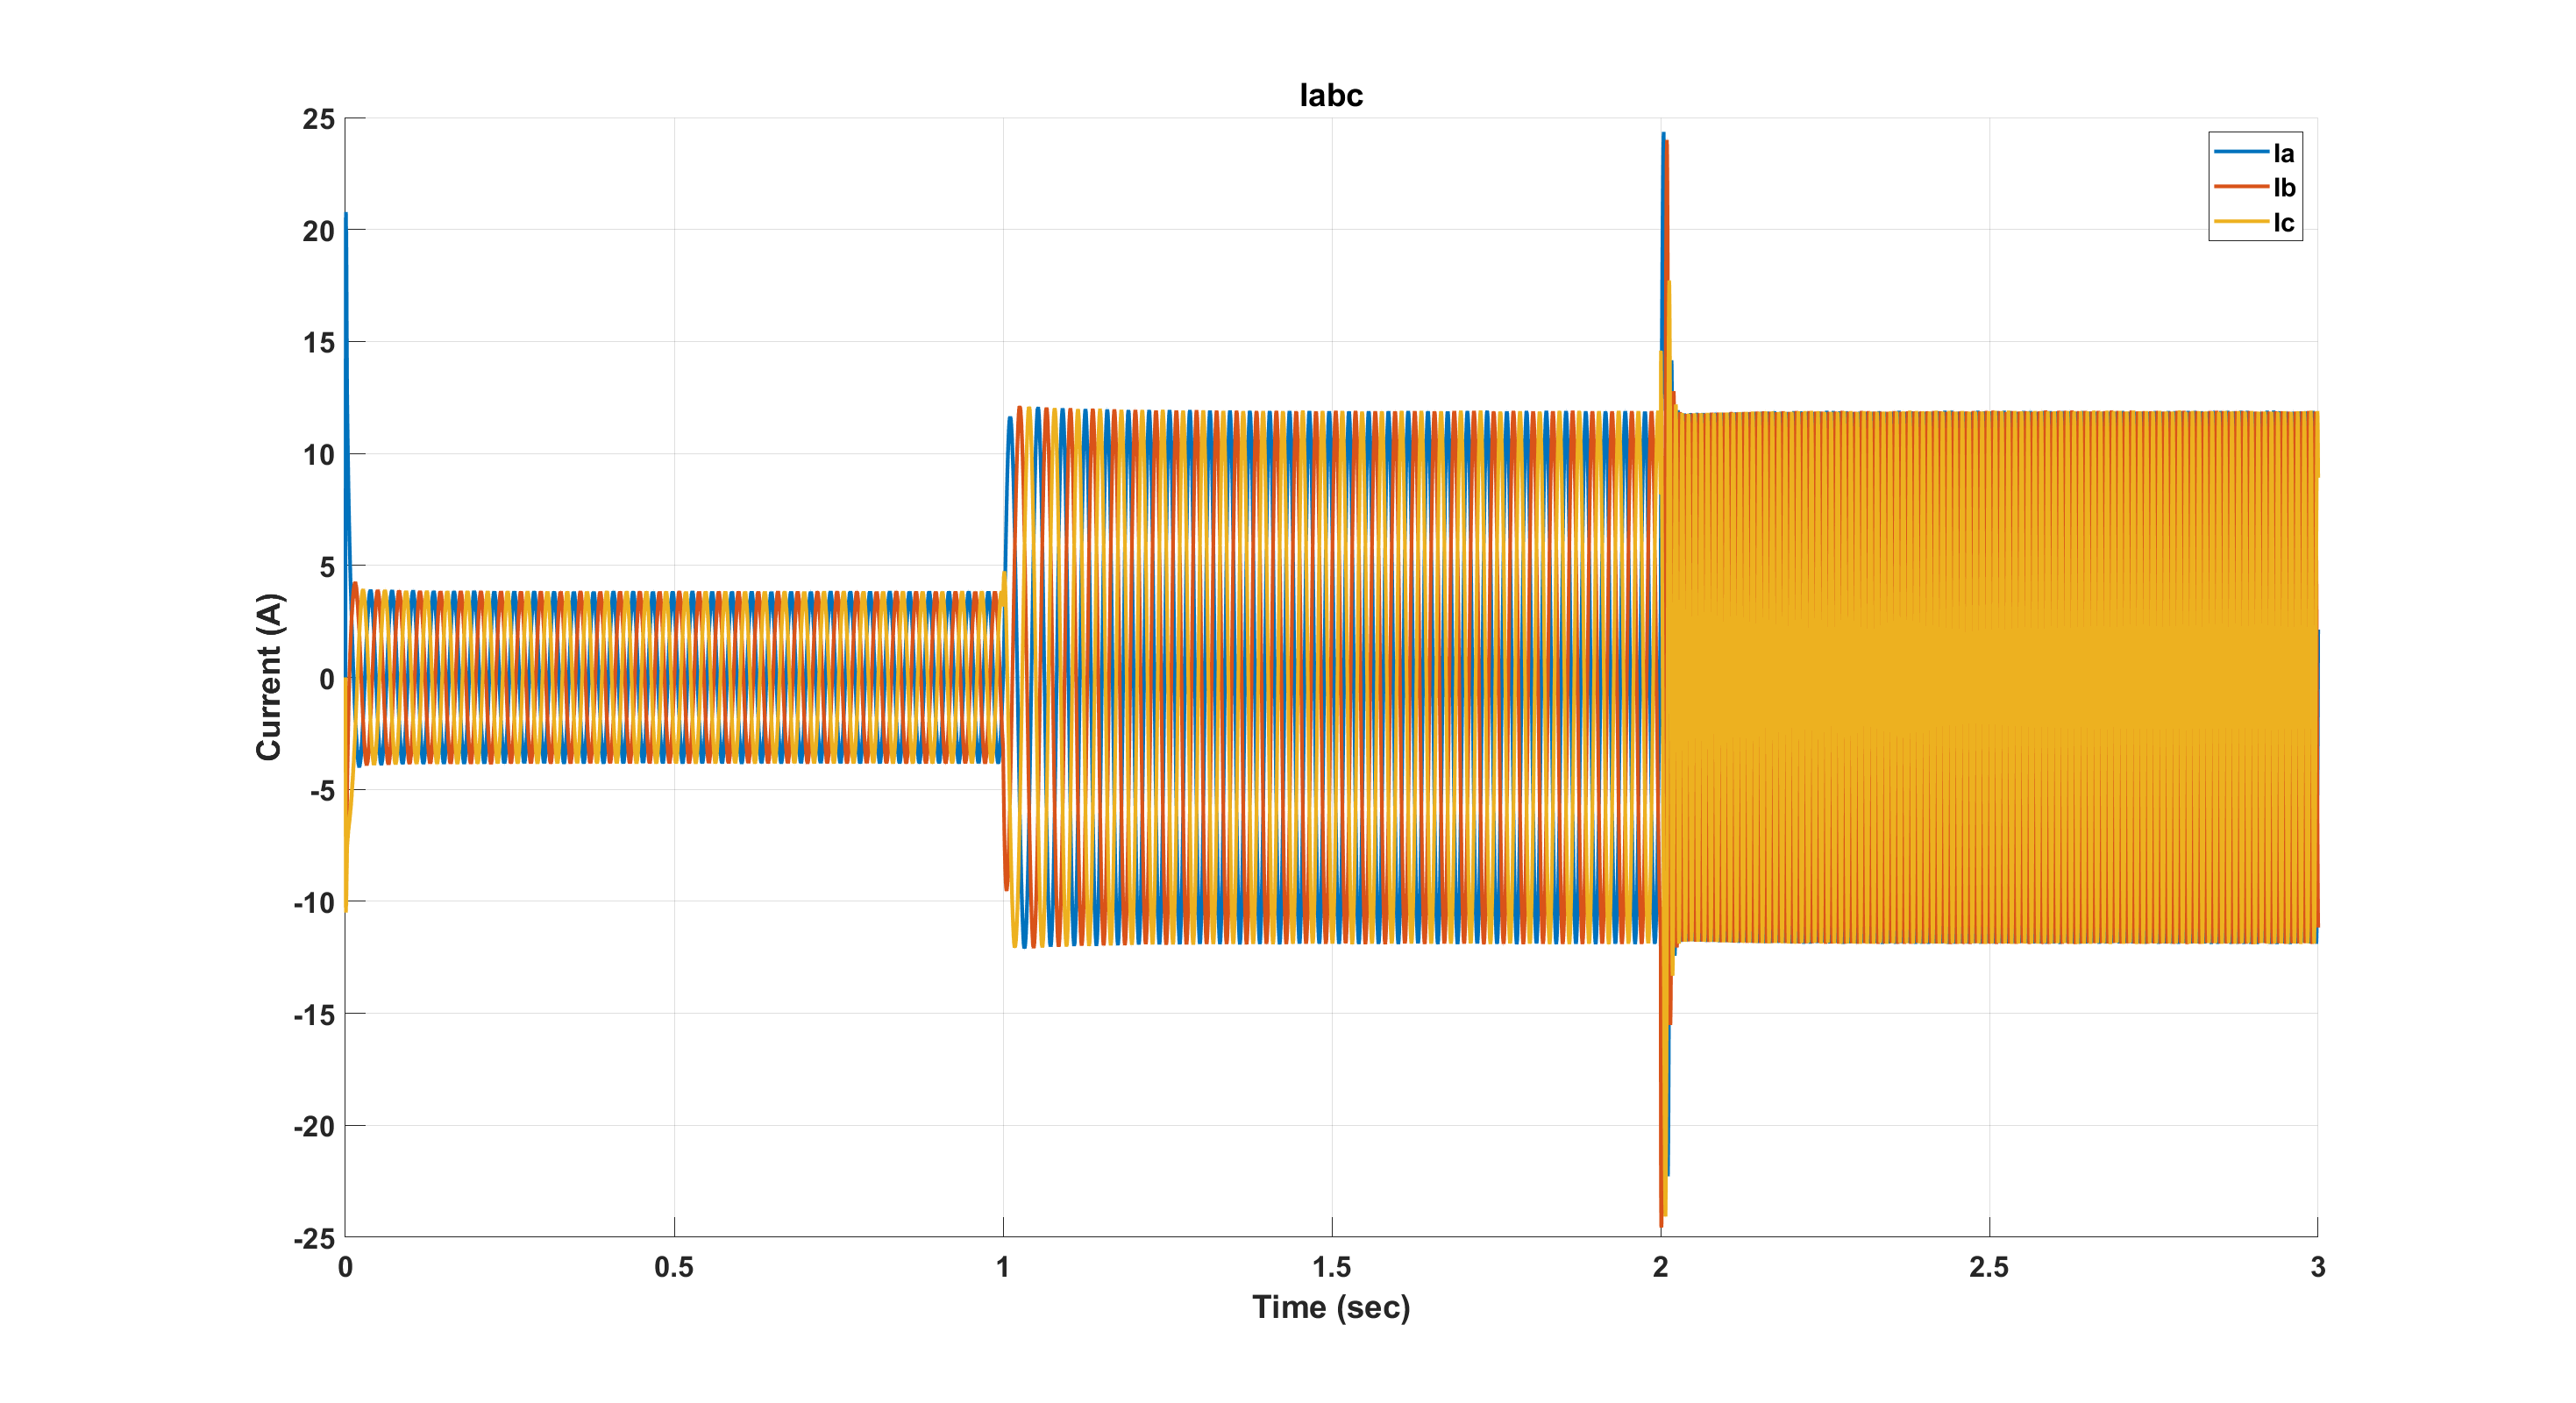
\includegraphics[scale=0.35]{SimulationResults/one_module/Iabc.eps}
\caption{abc Phase Currents for Healthy One Module Operation}
\label{fig:PhaseCurrentsAbcOneModuleHealthy}
\end{figure}

\begin{figure}[h!]
\centering
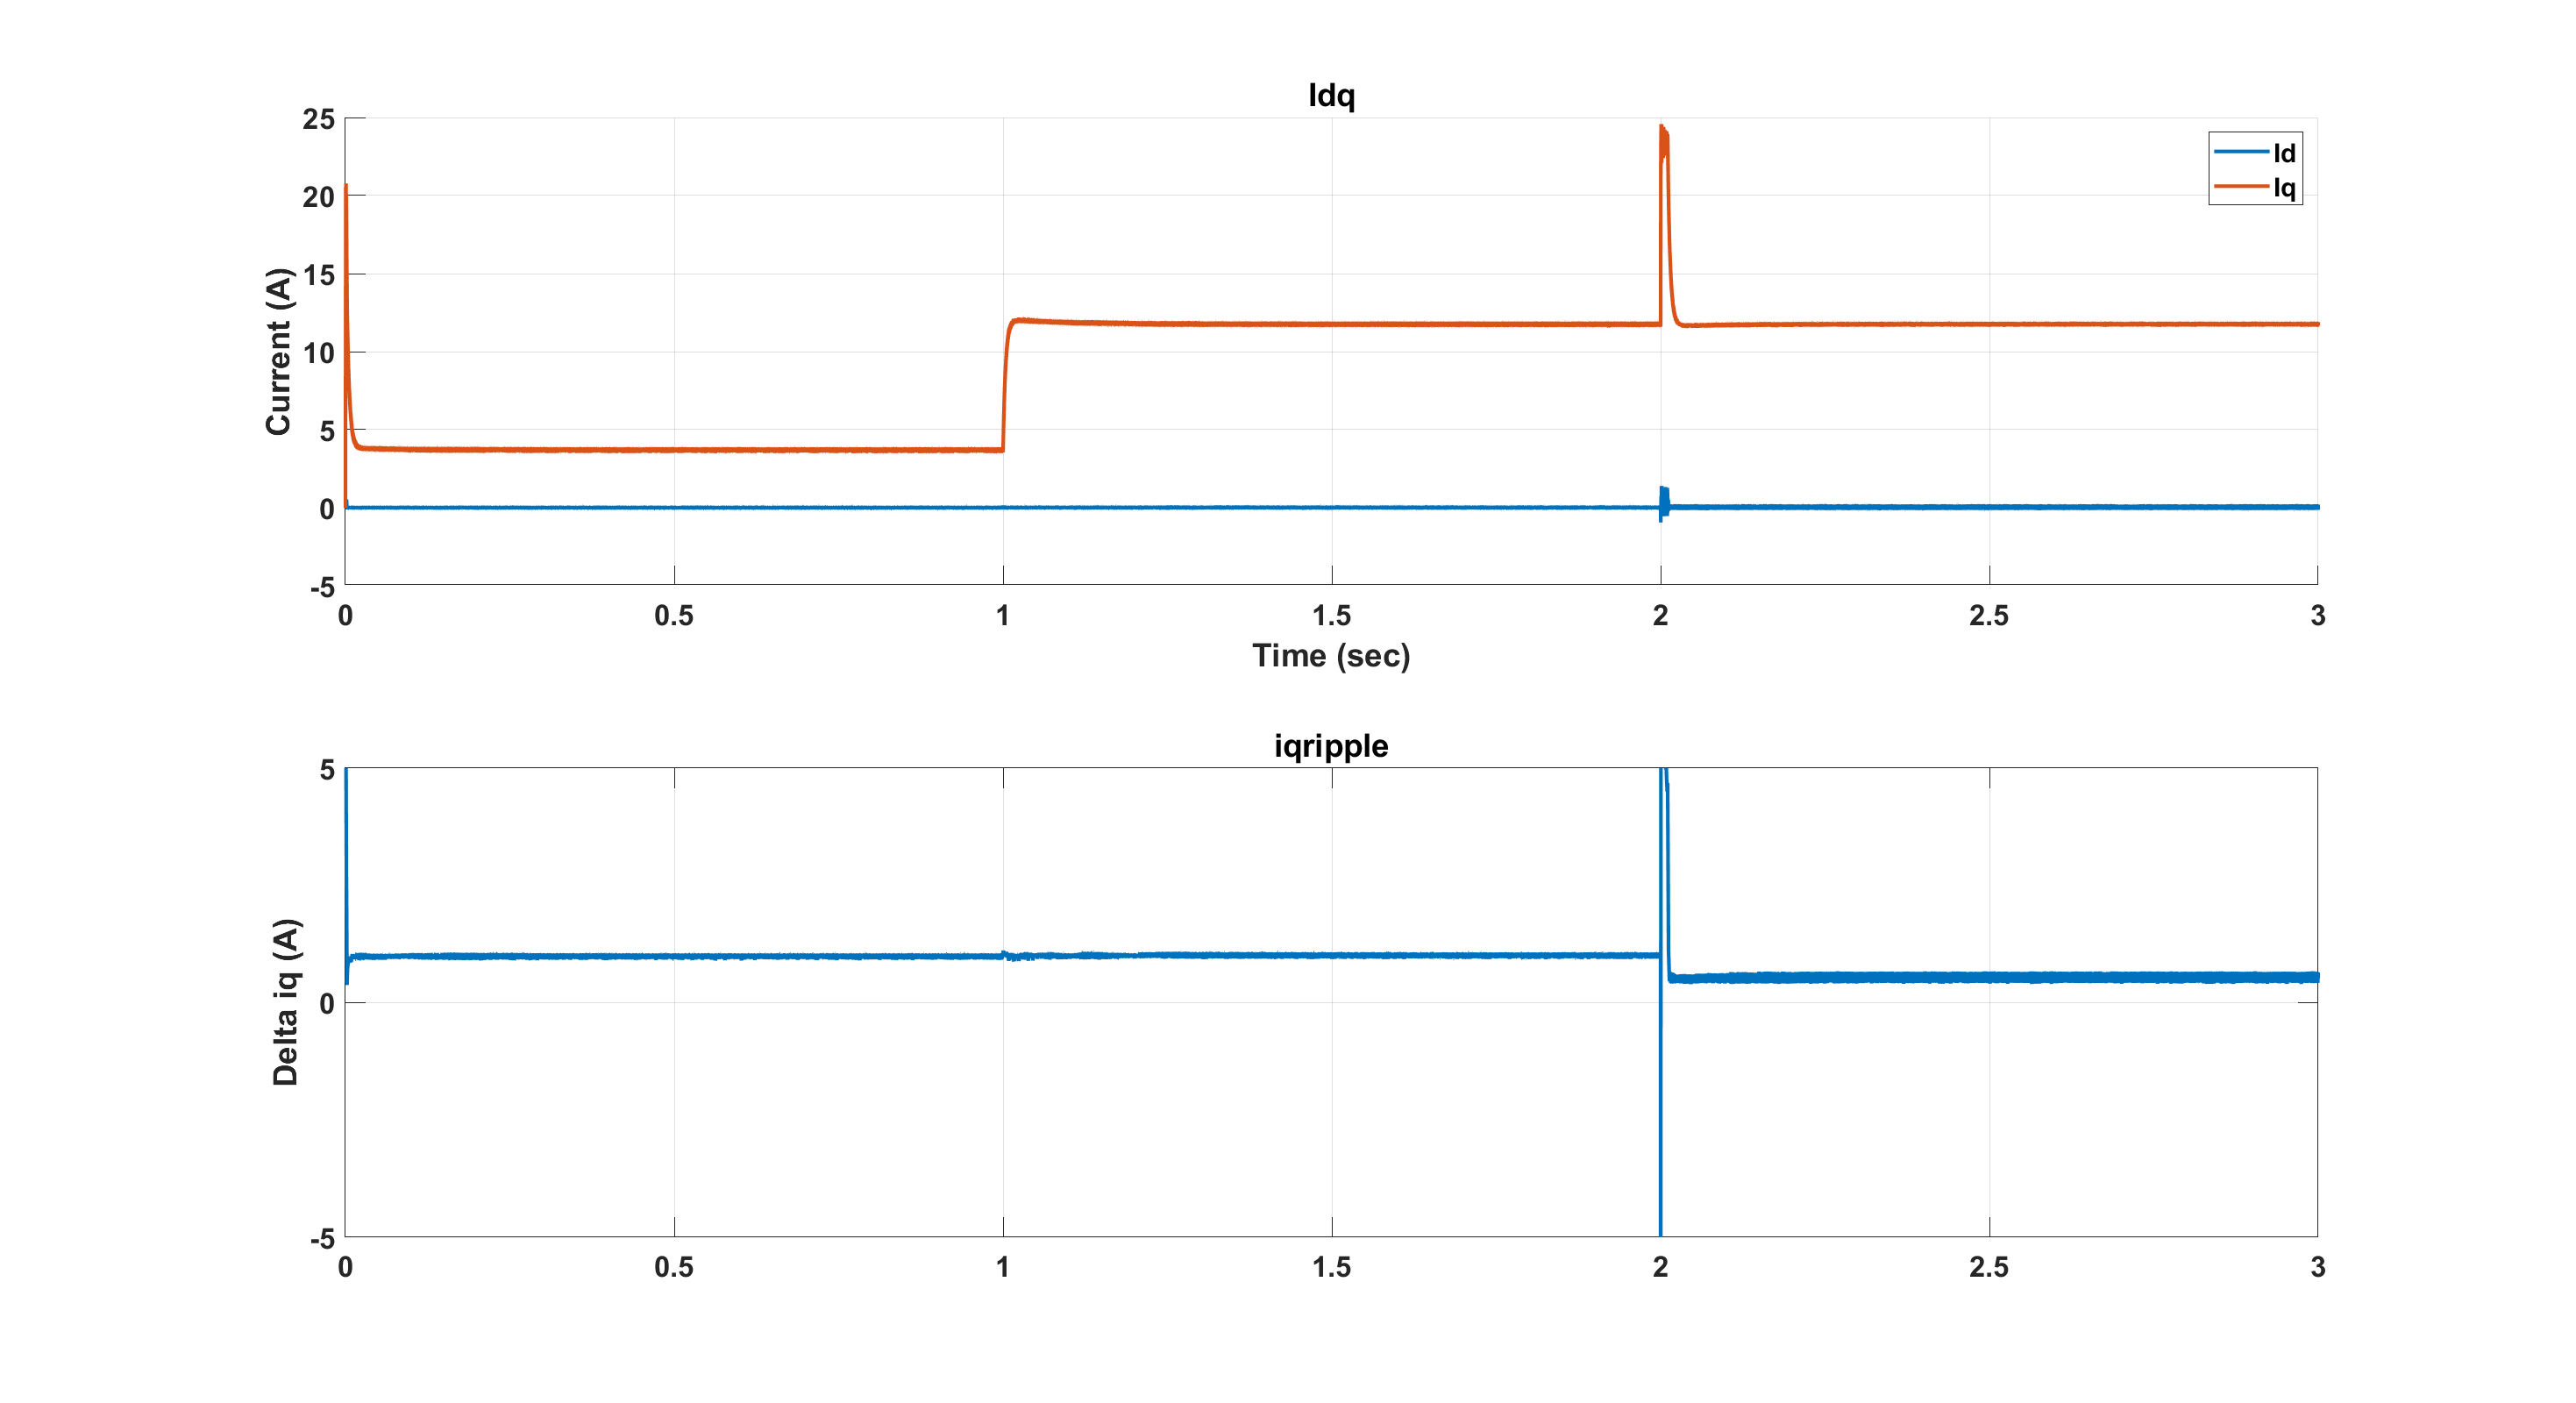
\includegraphics[scale=0.35]{SimulationResults/one_module/Idq_iqripple.eps}
\caption{dq Phase Currents and Iq Ripple Estimation for Healthy One Module Operation}
\label{fig:PhaseCurrentsDqOneModuleHealthy}
\end{figure}

\begin{figure}[h!]
\centering
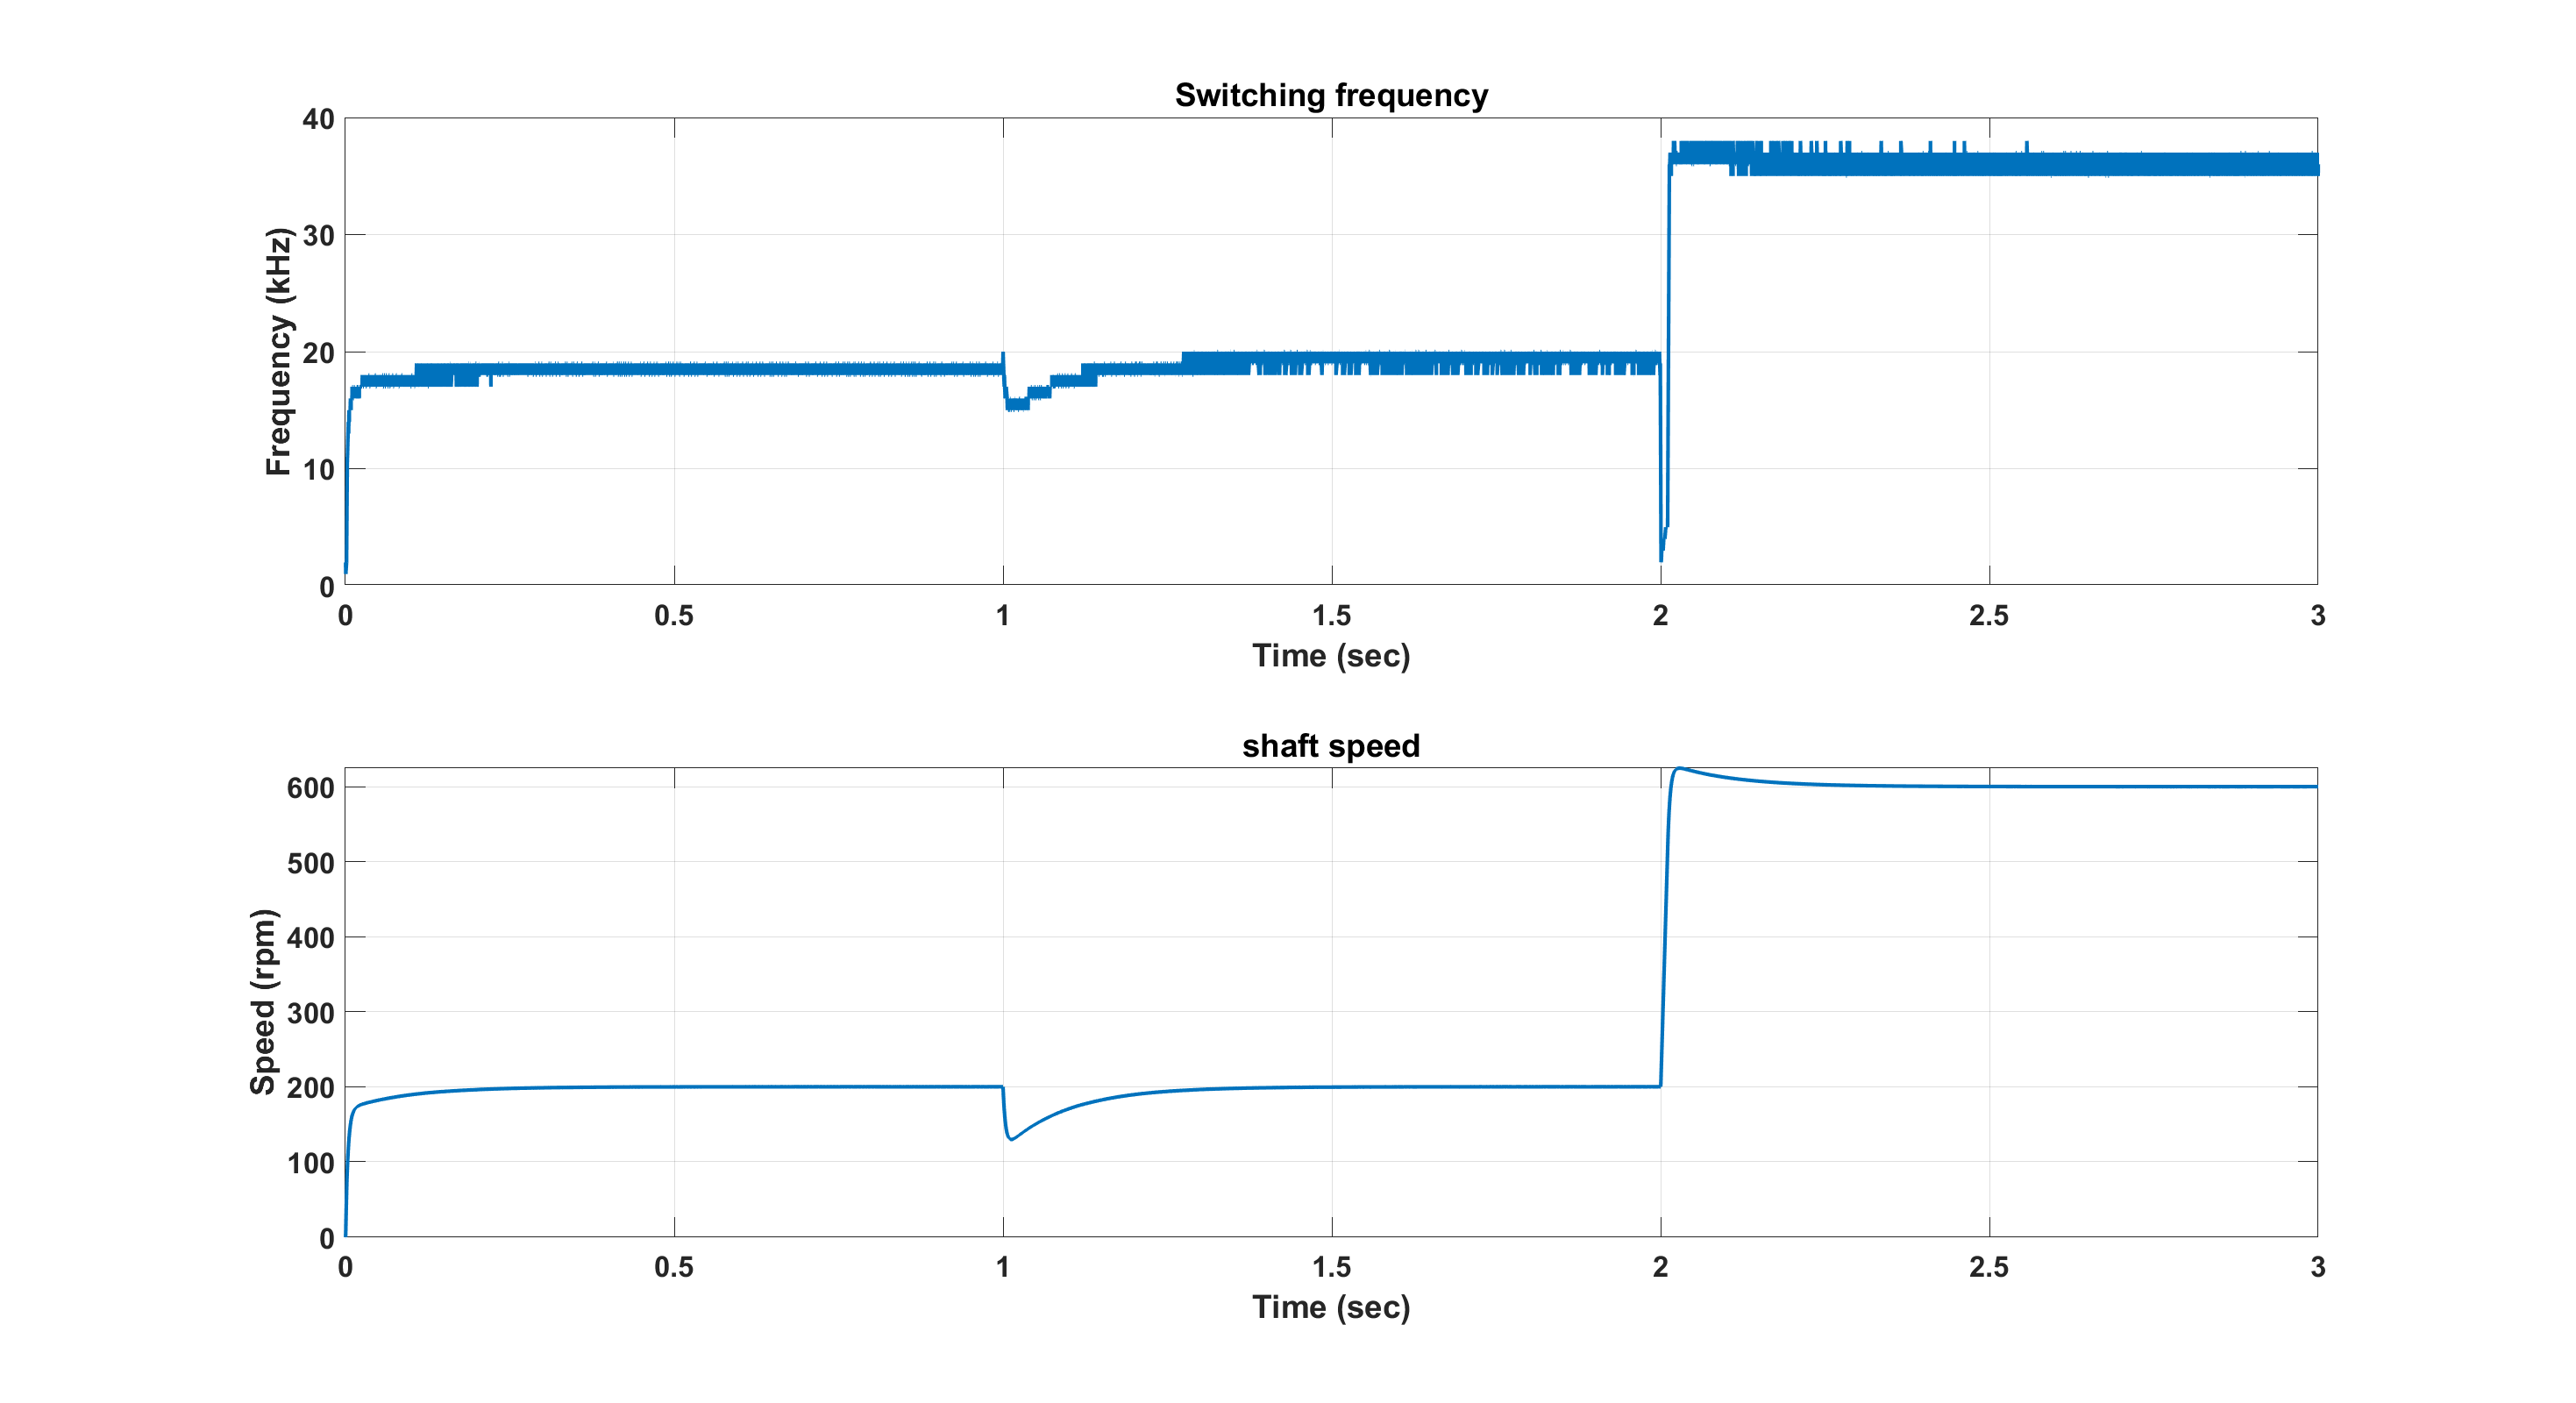
\includegraphics[scale=0.35]{SimulationResults/one_module/speed_fsw.eps}
\caption{Shaft Speed and Switching Frequency for Healthy One Module Operation}
\label{fig:ShaftSpeedFswOneModuleHealthy}
\end{figure}

\begin{figure}[h!]
\centering
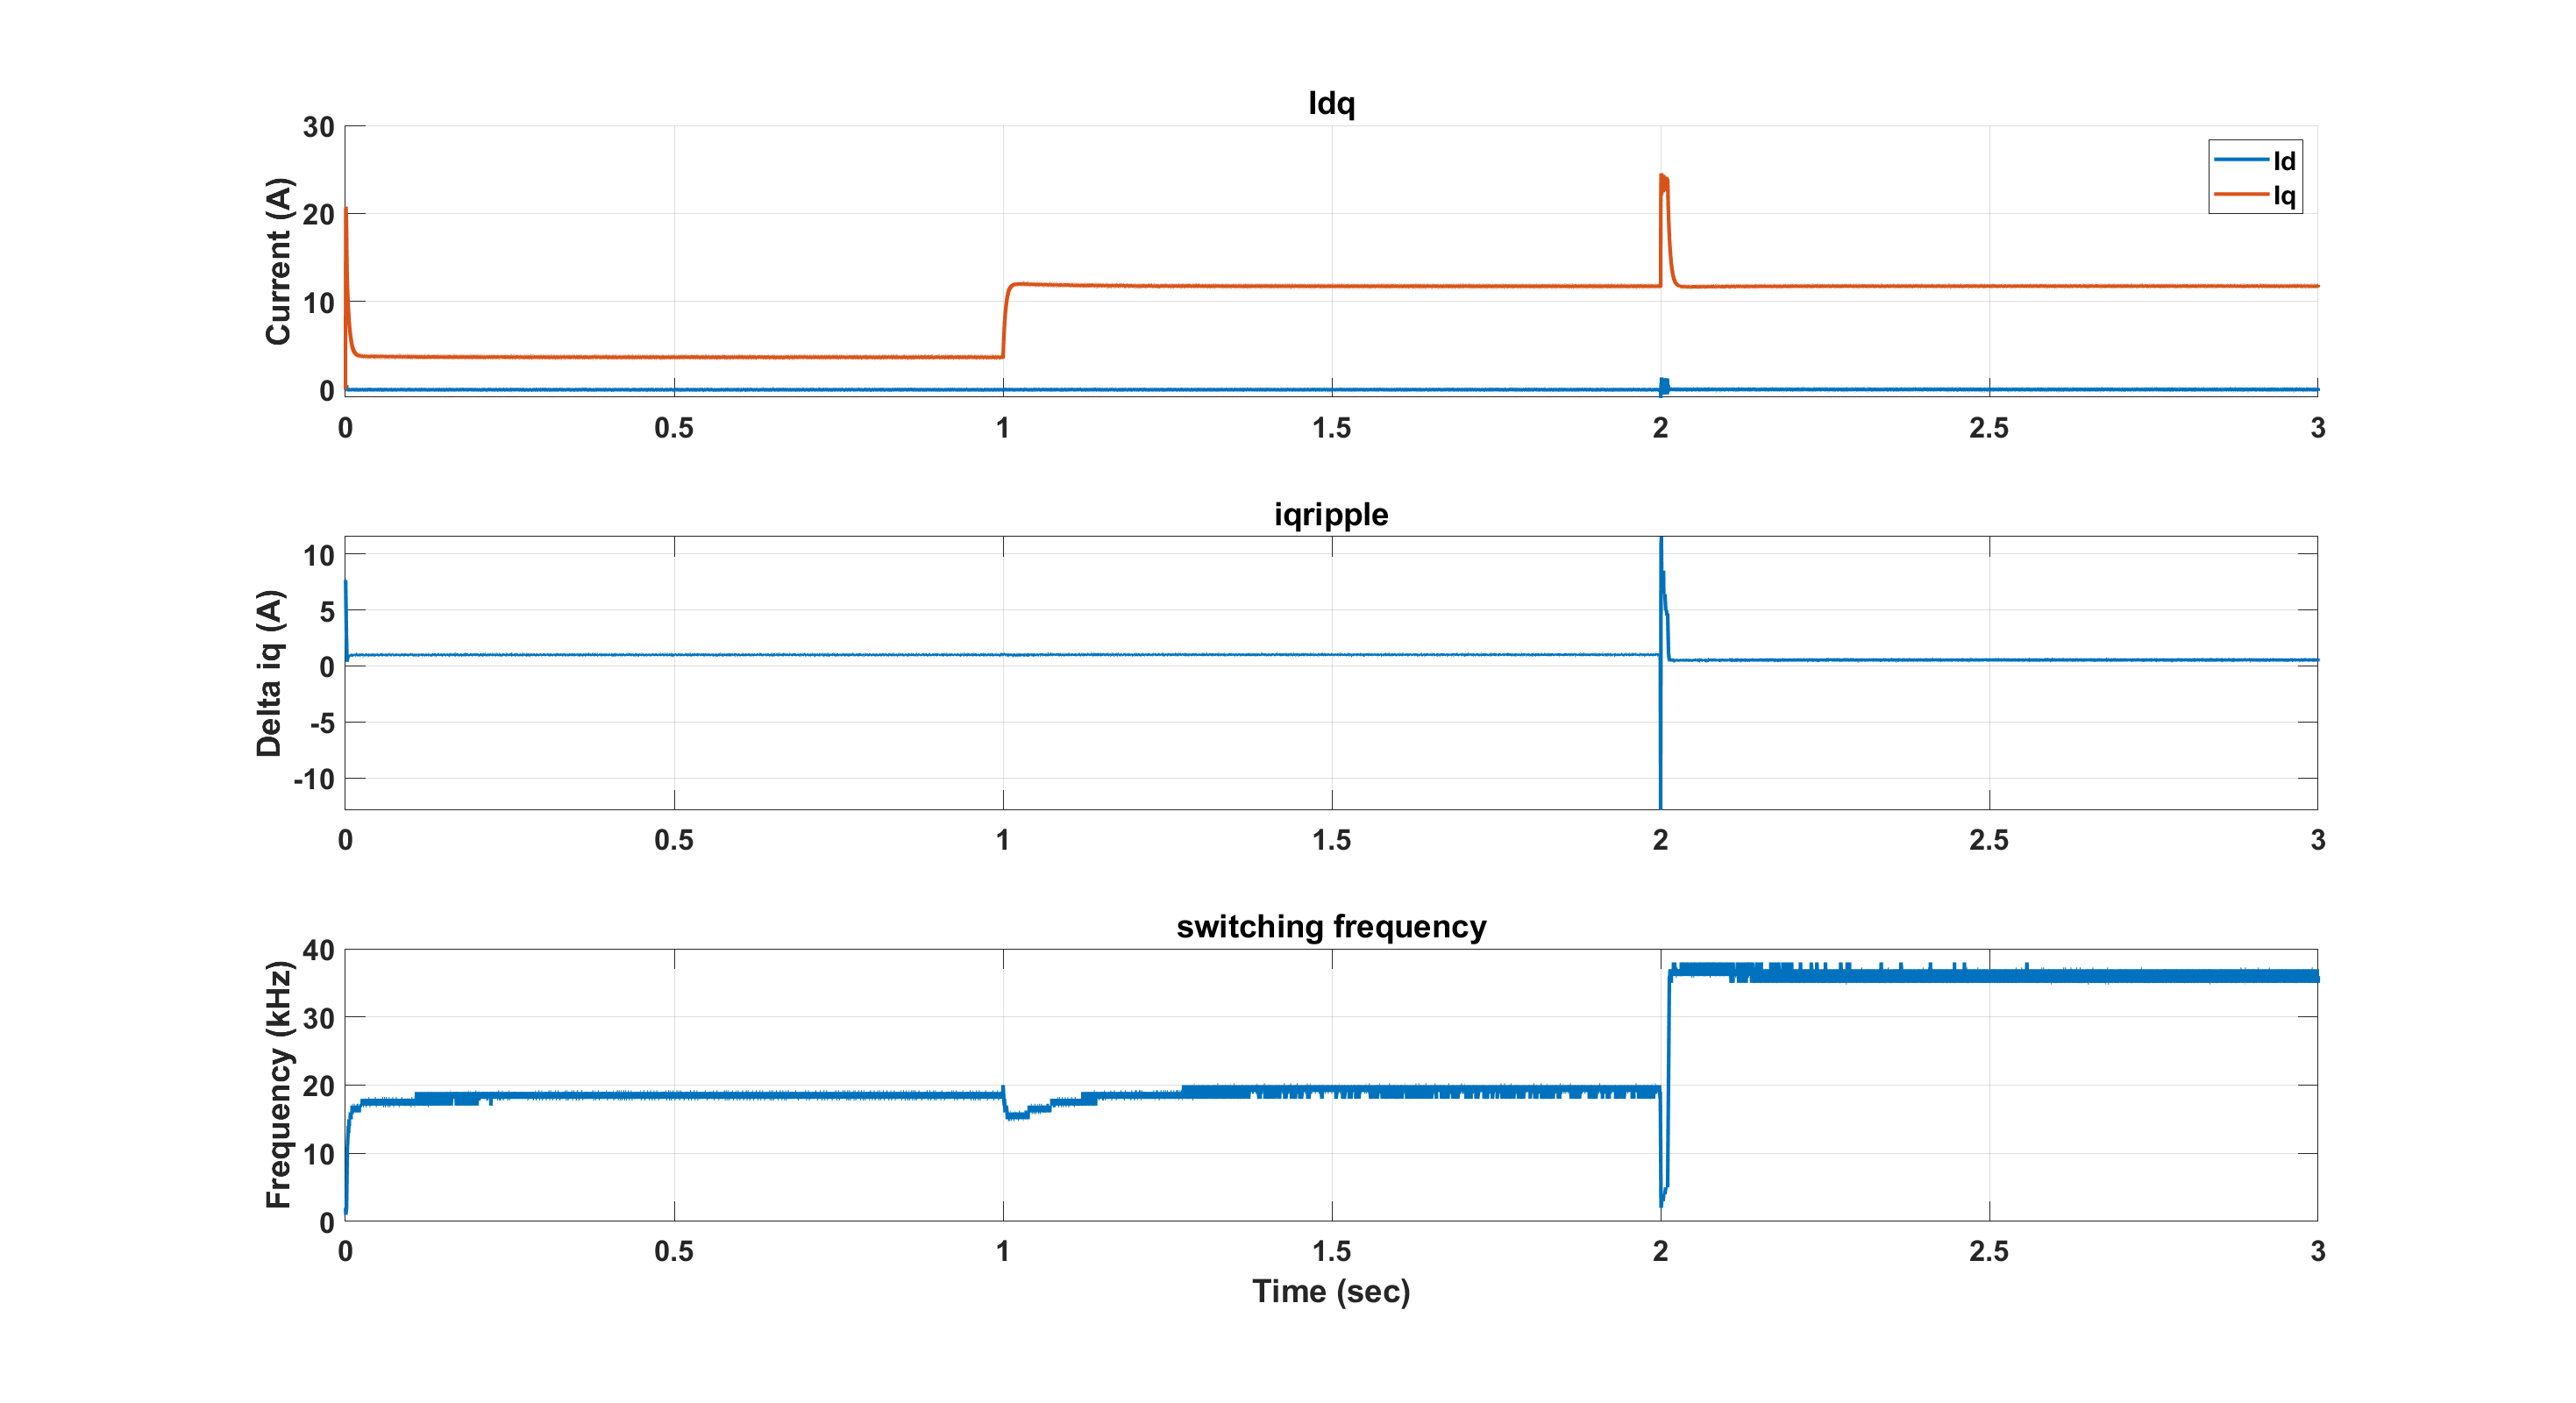
\includegraphics[scale=0.35]{SimulationResults/one_module/te_iqripple_fsw.eps}
\caption{Torque, Iq Ripple and Switching Frequency for Healthy One Module Operation}
\label{fig:TorqueIqrippleFswOneModuleHealthy}
\end{figure}

\begin{figure}[h!]
\centering
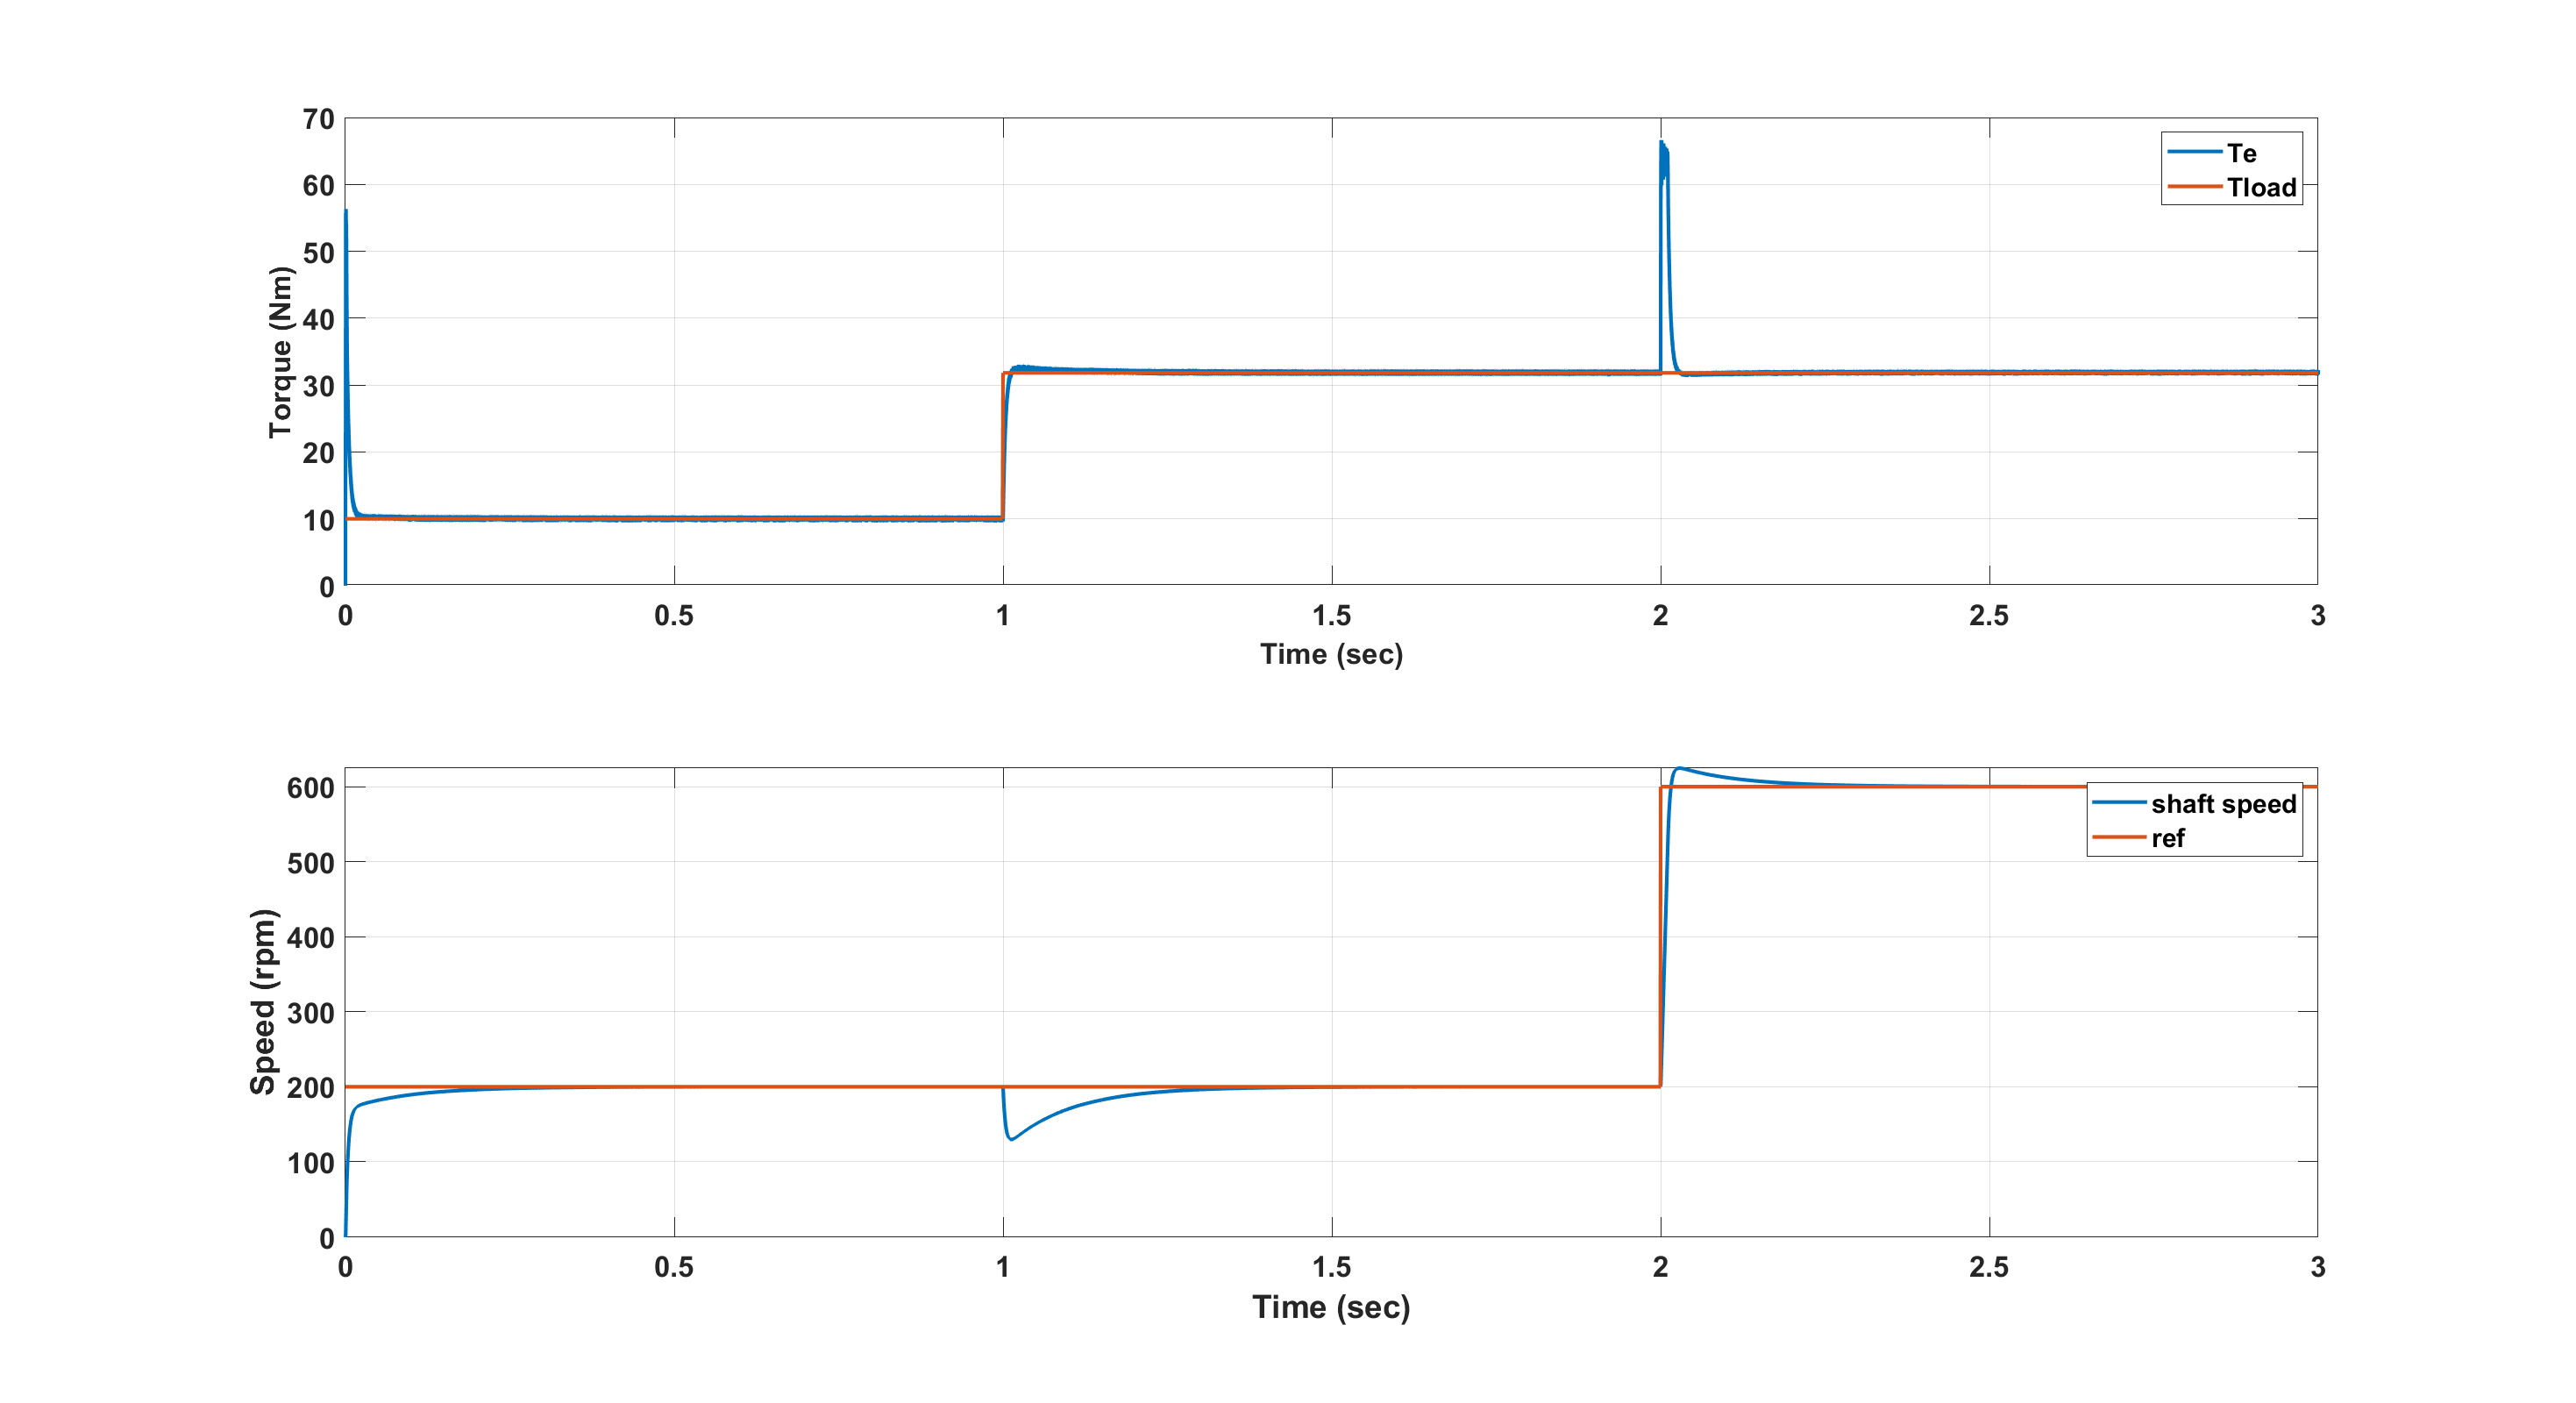
\includegraphics[scale=0.35]{SimulationResults/one_module/te_speed.eps}
\caption{Torque and Shaft Speed for Healthy One Module Operation}
\label{fig:TorqueShaftSpeedOneModuleHealthy}
\end{figure}

\section{Two Modules}
\subsection{Healthy Operation}
This section contains informations.

\begin{figure}[h!]
\centering
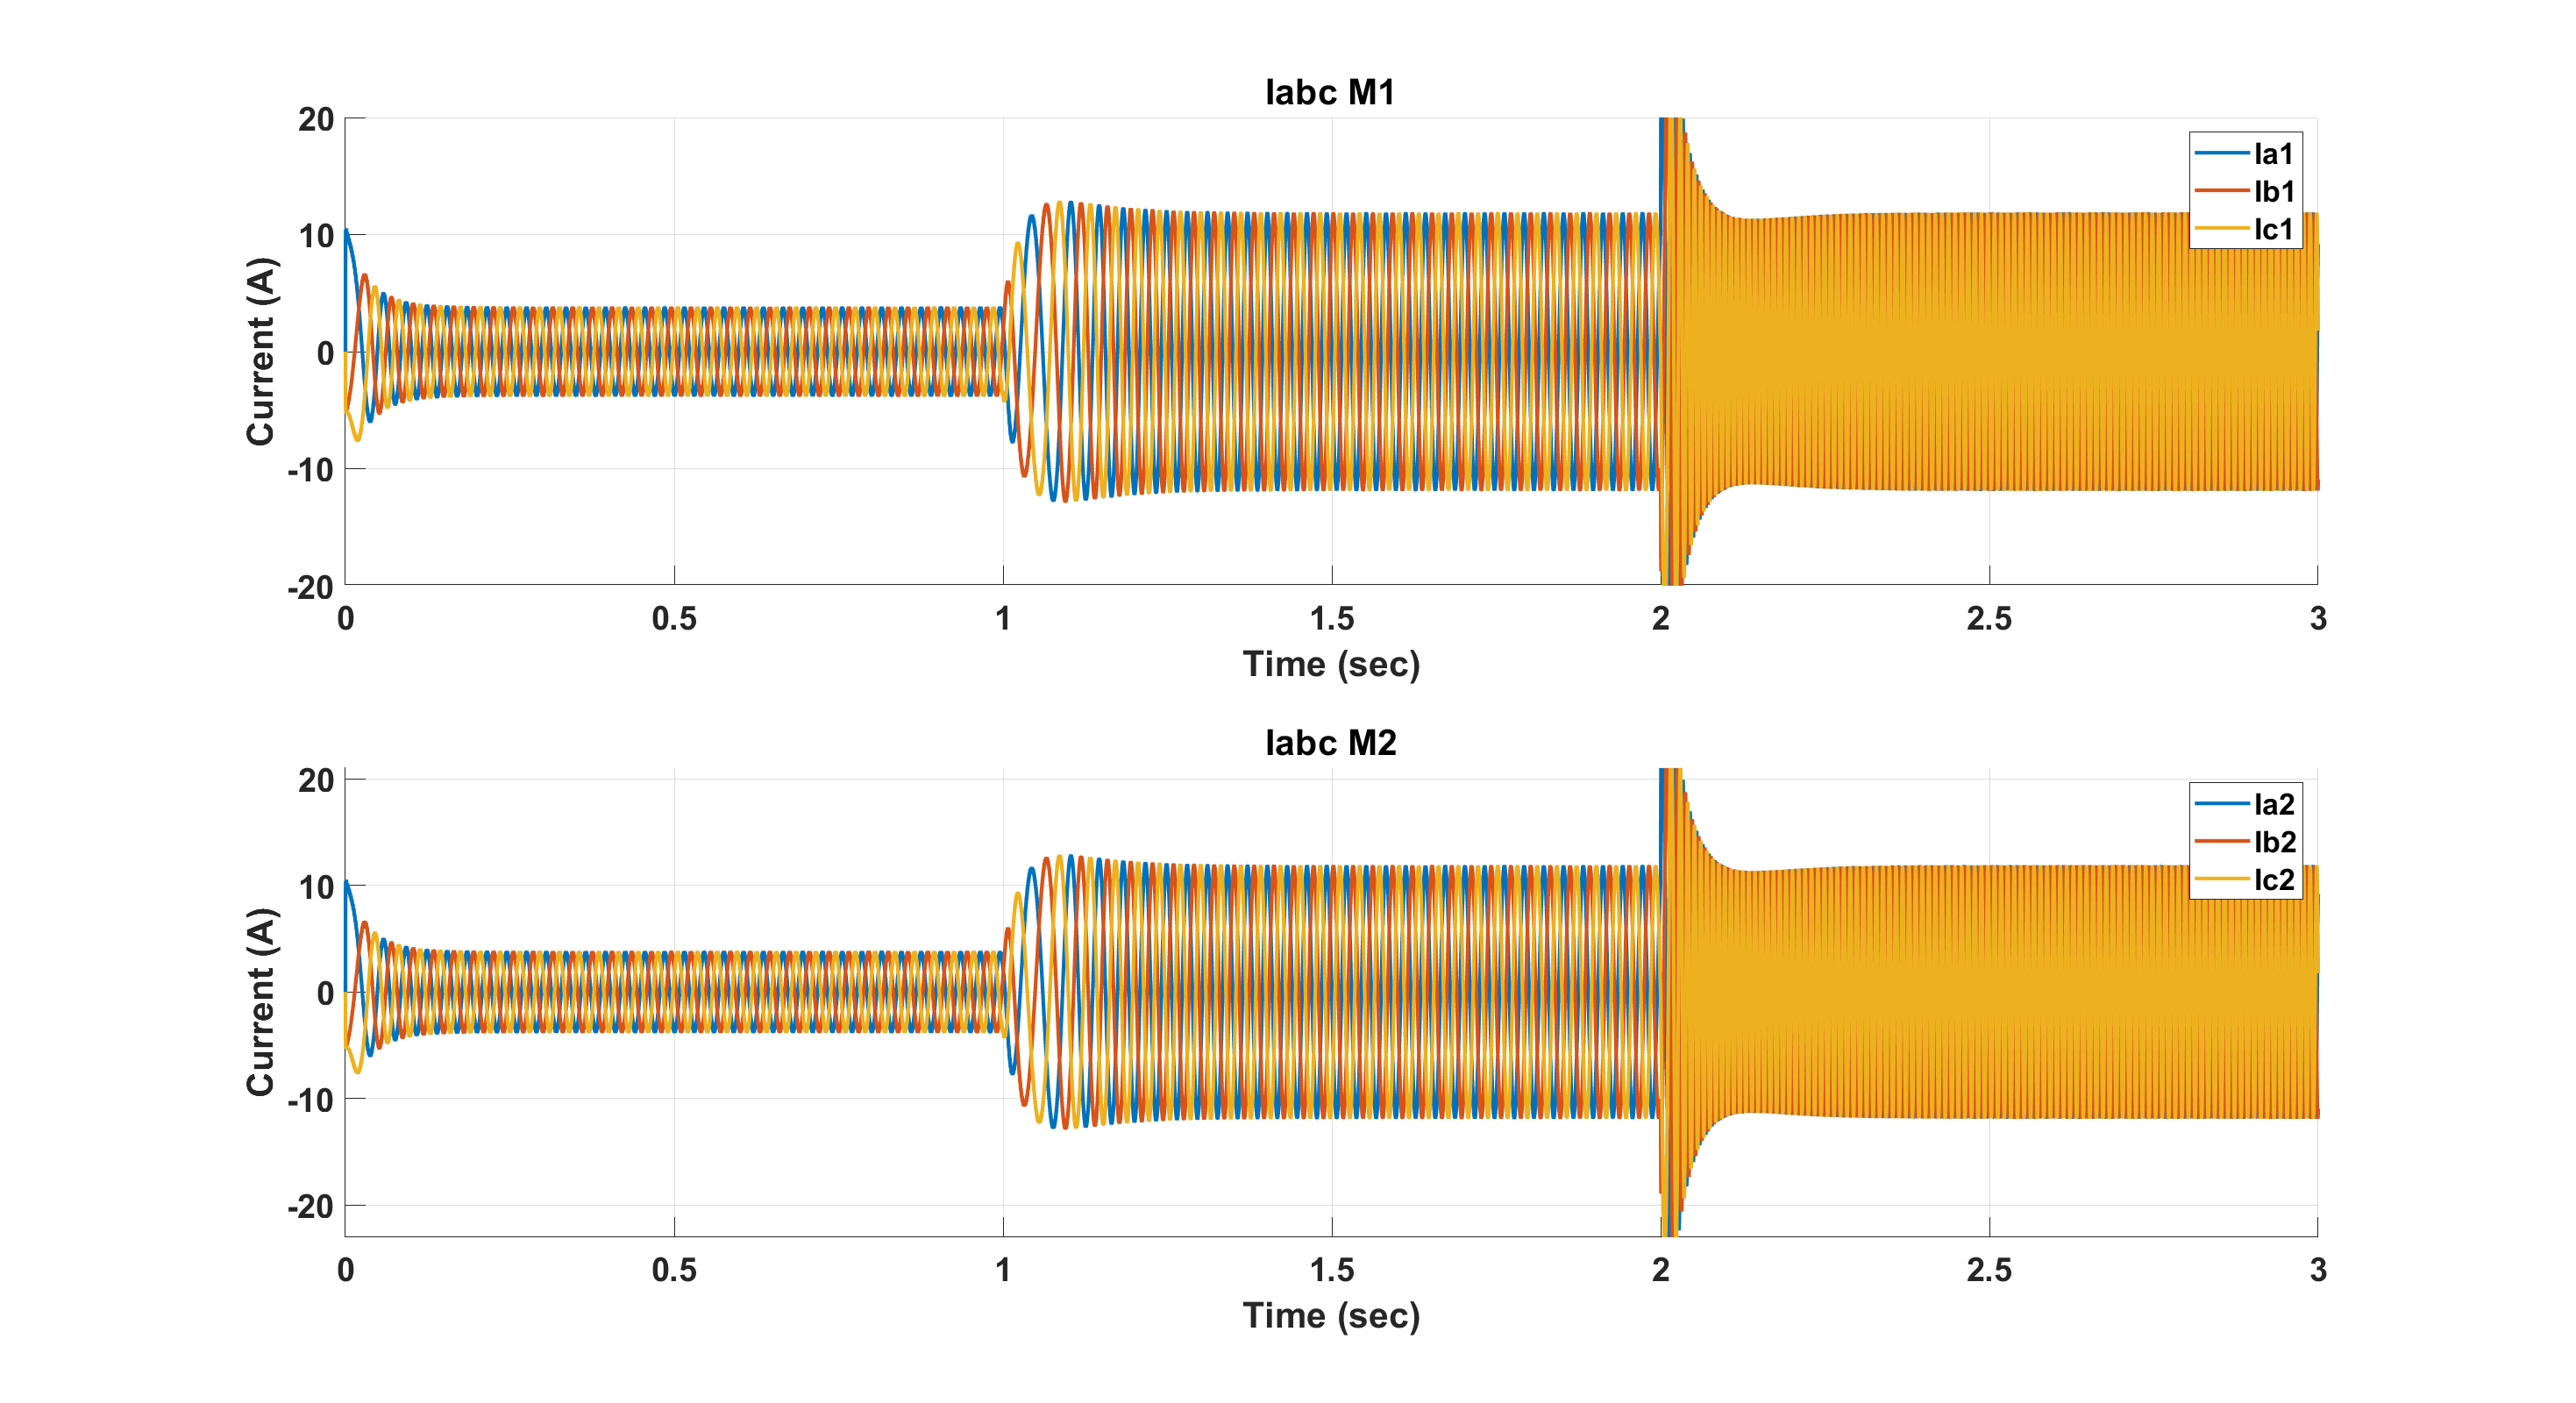
\includegraphics[scale=0.35]{SimulationResults/two_modules/healthy/Iabc.eps}
\caption{abc Phase Currents for Healthy Two Modules Operation}
\label{fig:PhaseCurrentsAbcTwoModulesHealthy}
\end{figure}

\begin{figure}[h!]
\centering
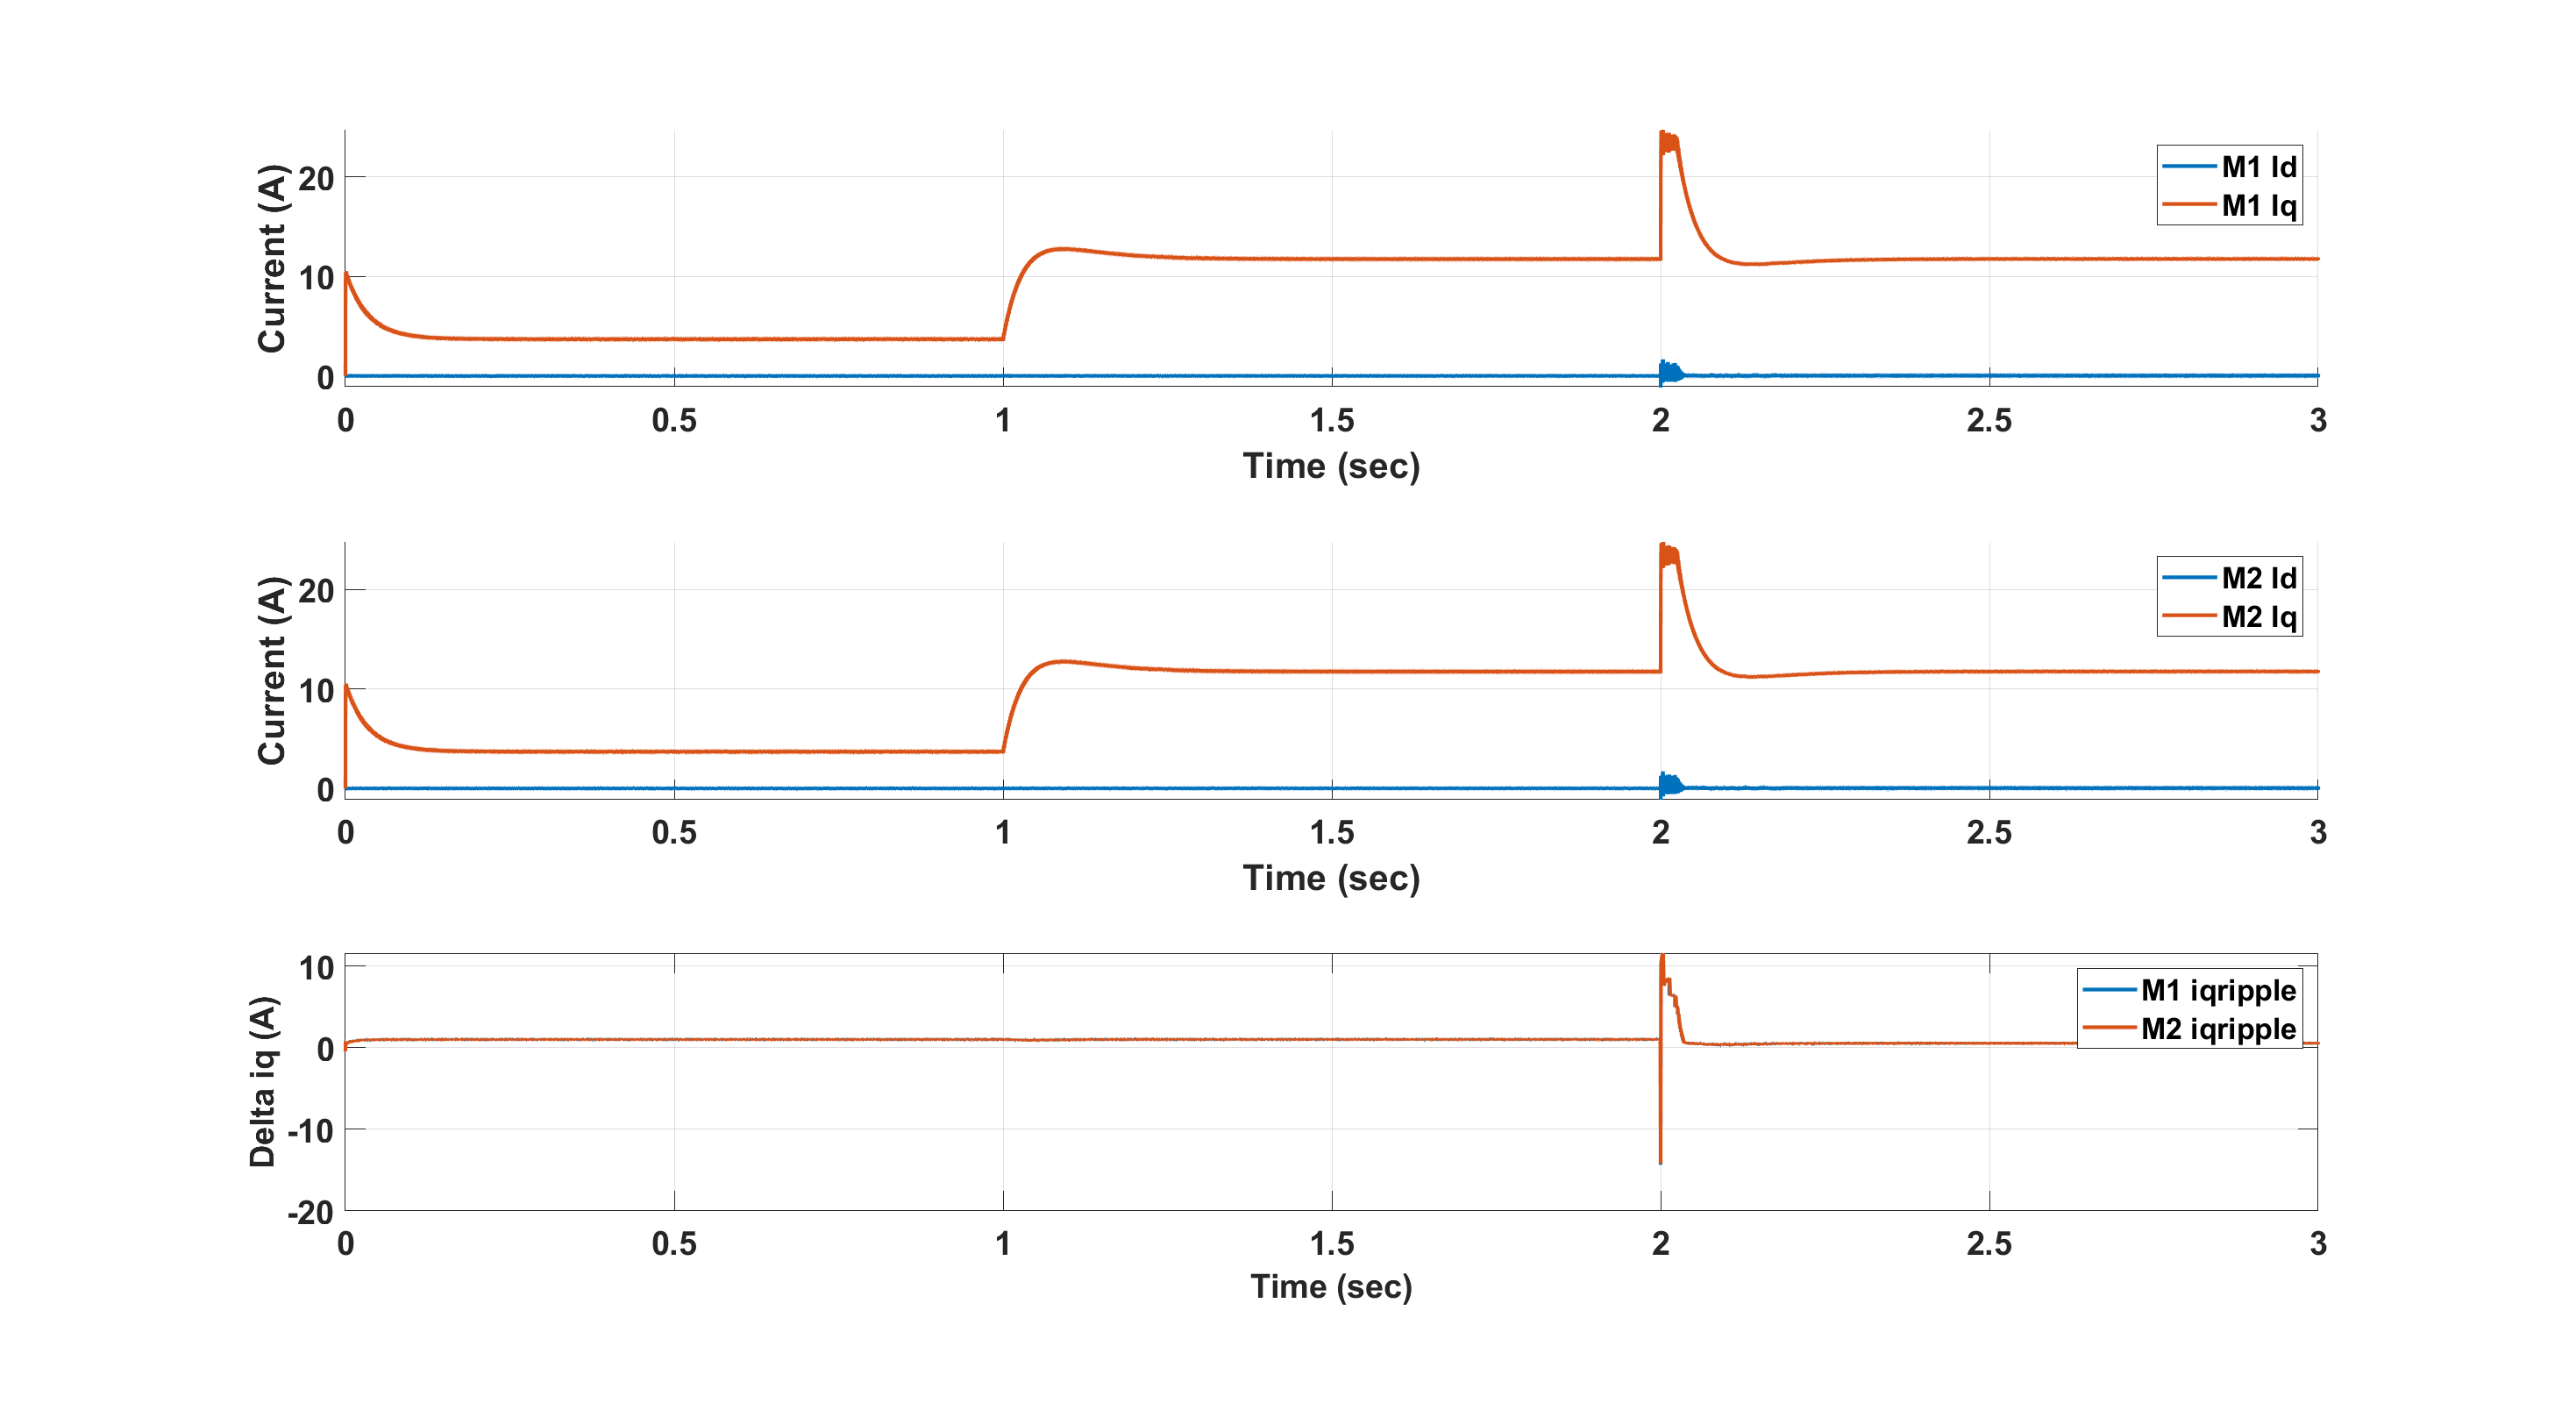
\includegraphics[scale=0.35]{SimulationResults/two_modules/healthy/Idq_iqripple.eps}
\caption{dq Phase Currents for Healthy Two Modules Operation}
\label{fig:PhaseCurrentsDqTwoModulesHealthy}
\end{figure}

\begin{figure}[h!]
\centering
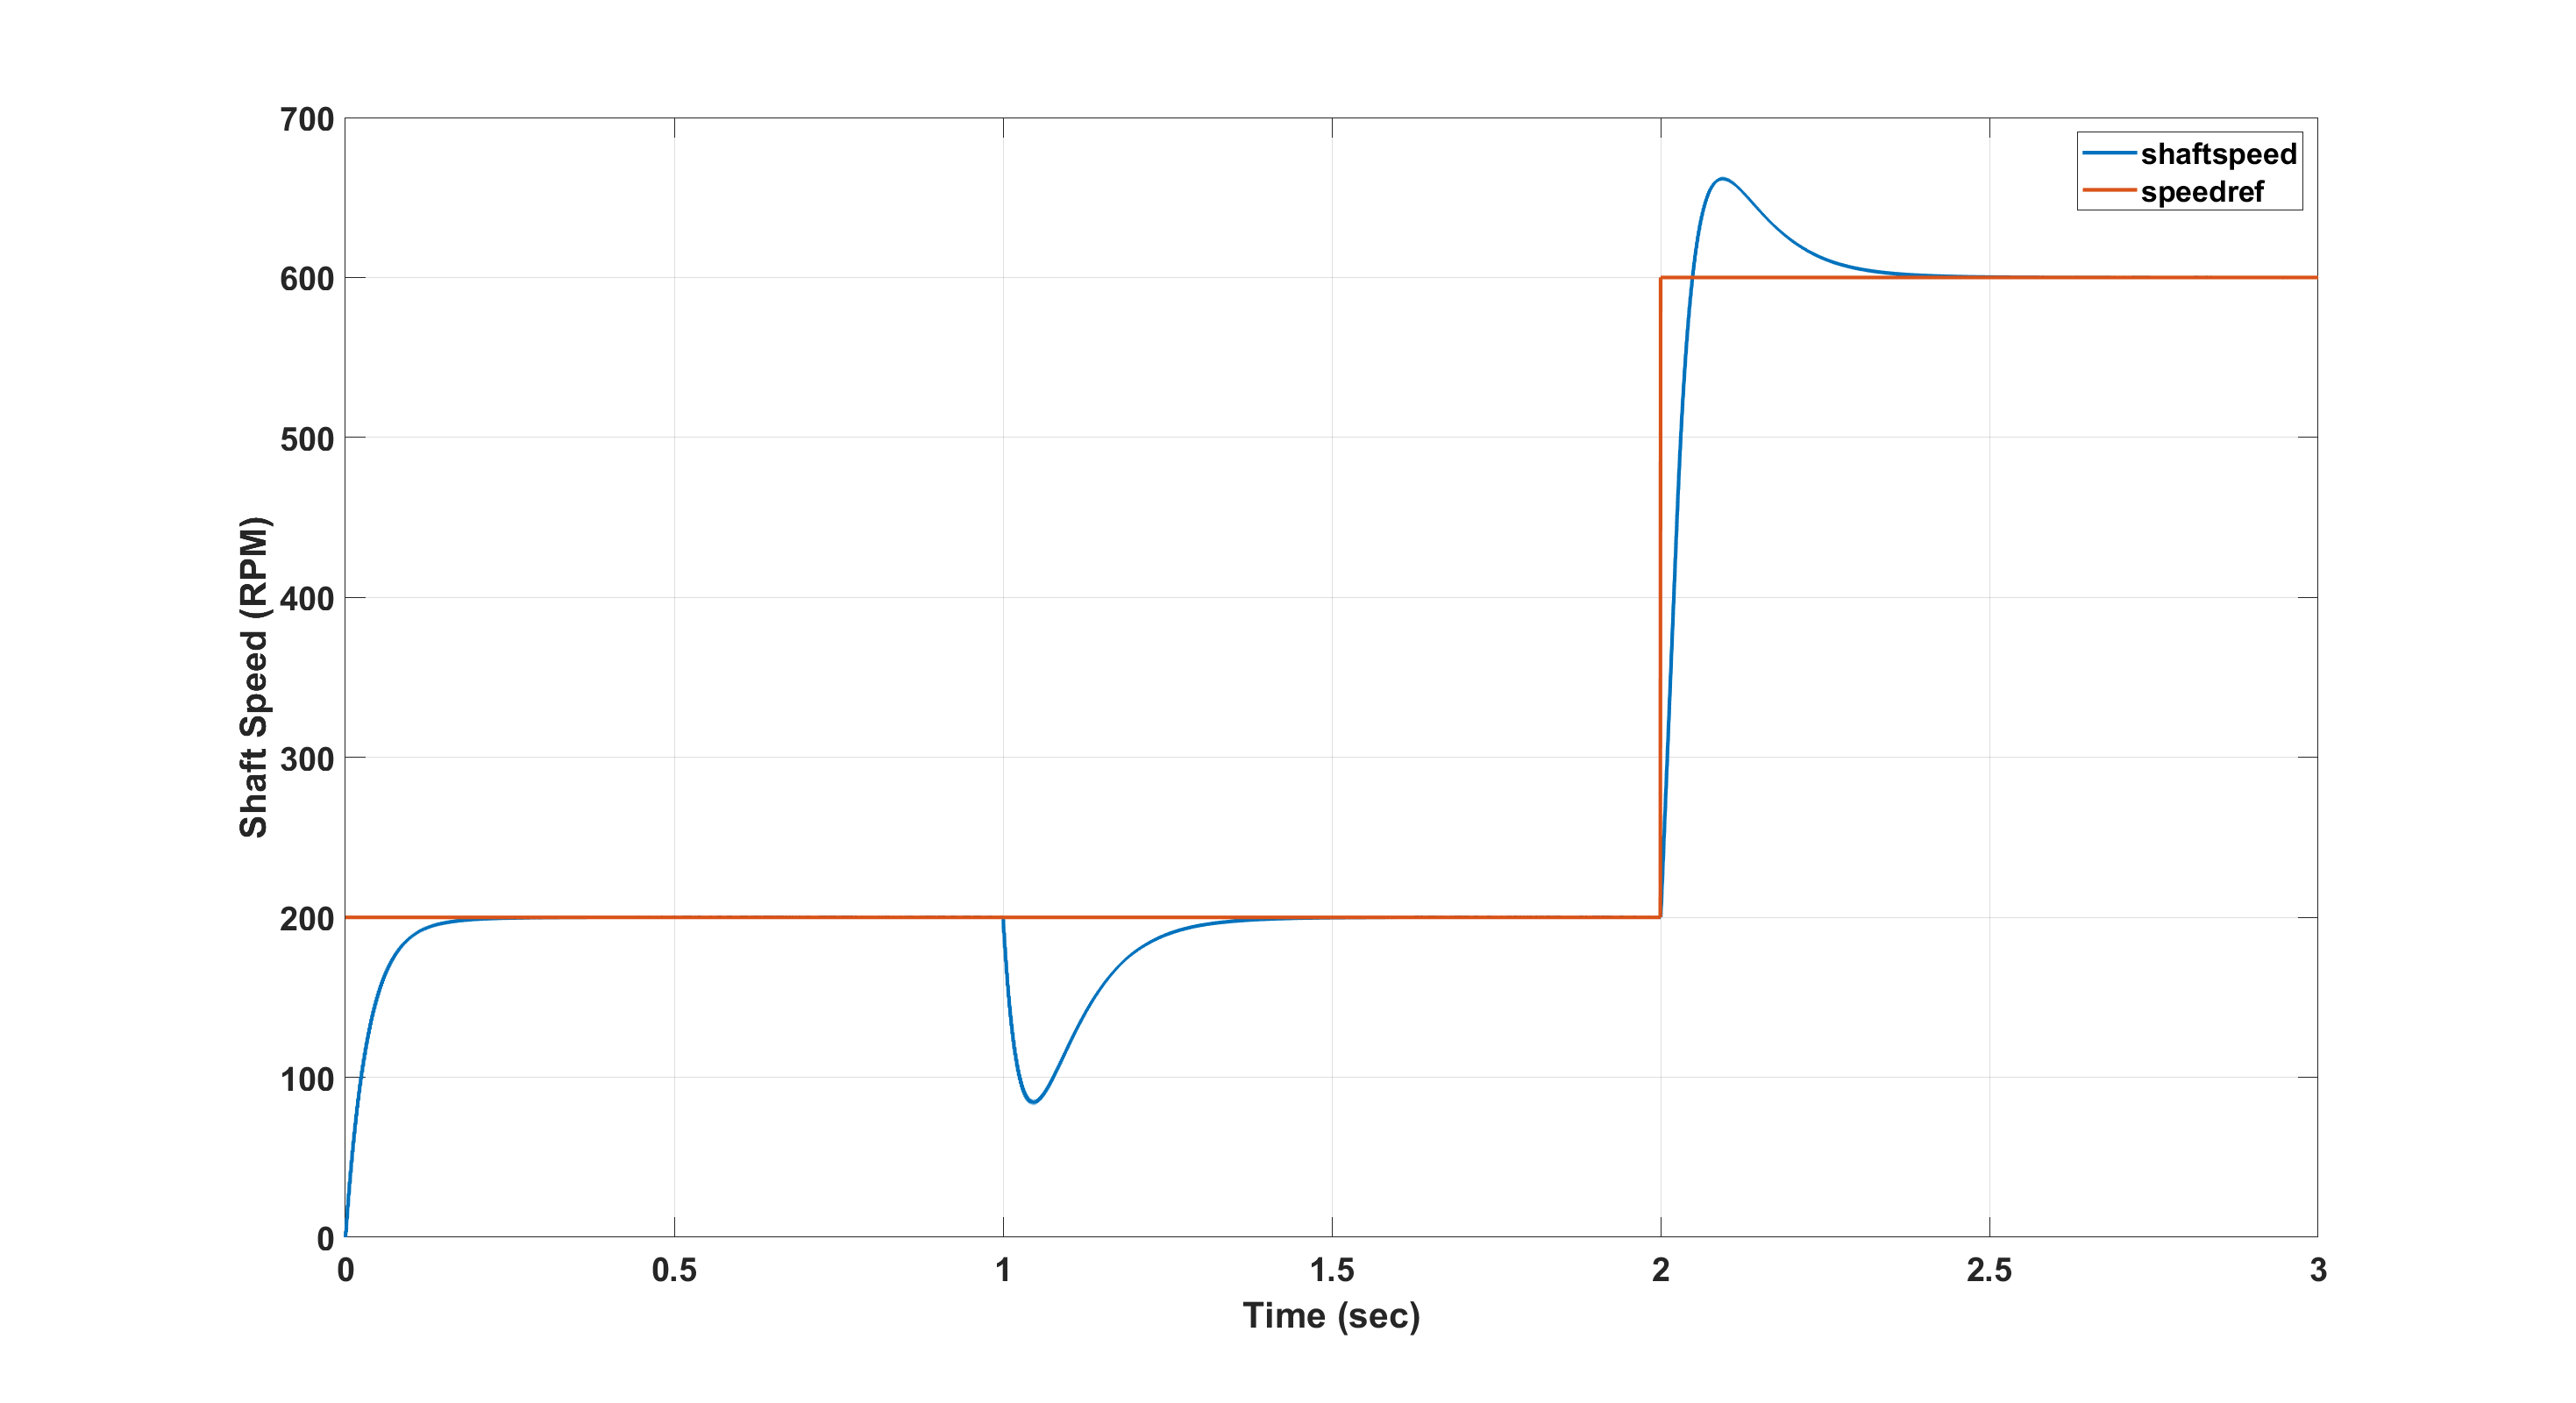
\includegraphics[scale=0.35]{SimulationResults/two_modules/healthy/speed.eps}
\caption{Shaft Speed for Healthy Two Modules Operation}
\label{fig:ShaftSpeedTwoModulesHealthy}
\end{figure}

\begin{figure}[h!]
\centering
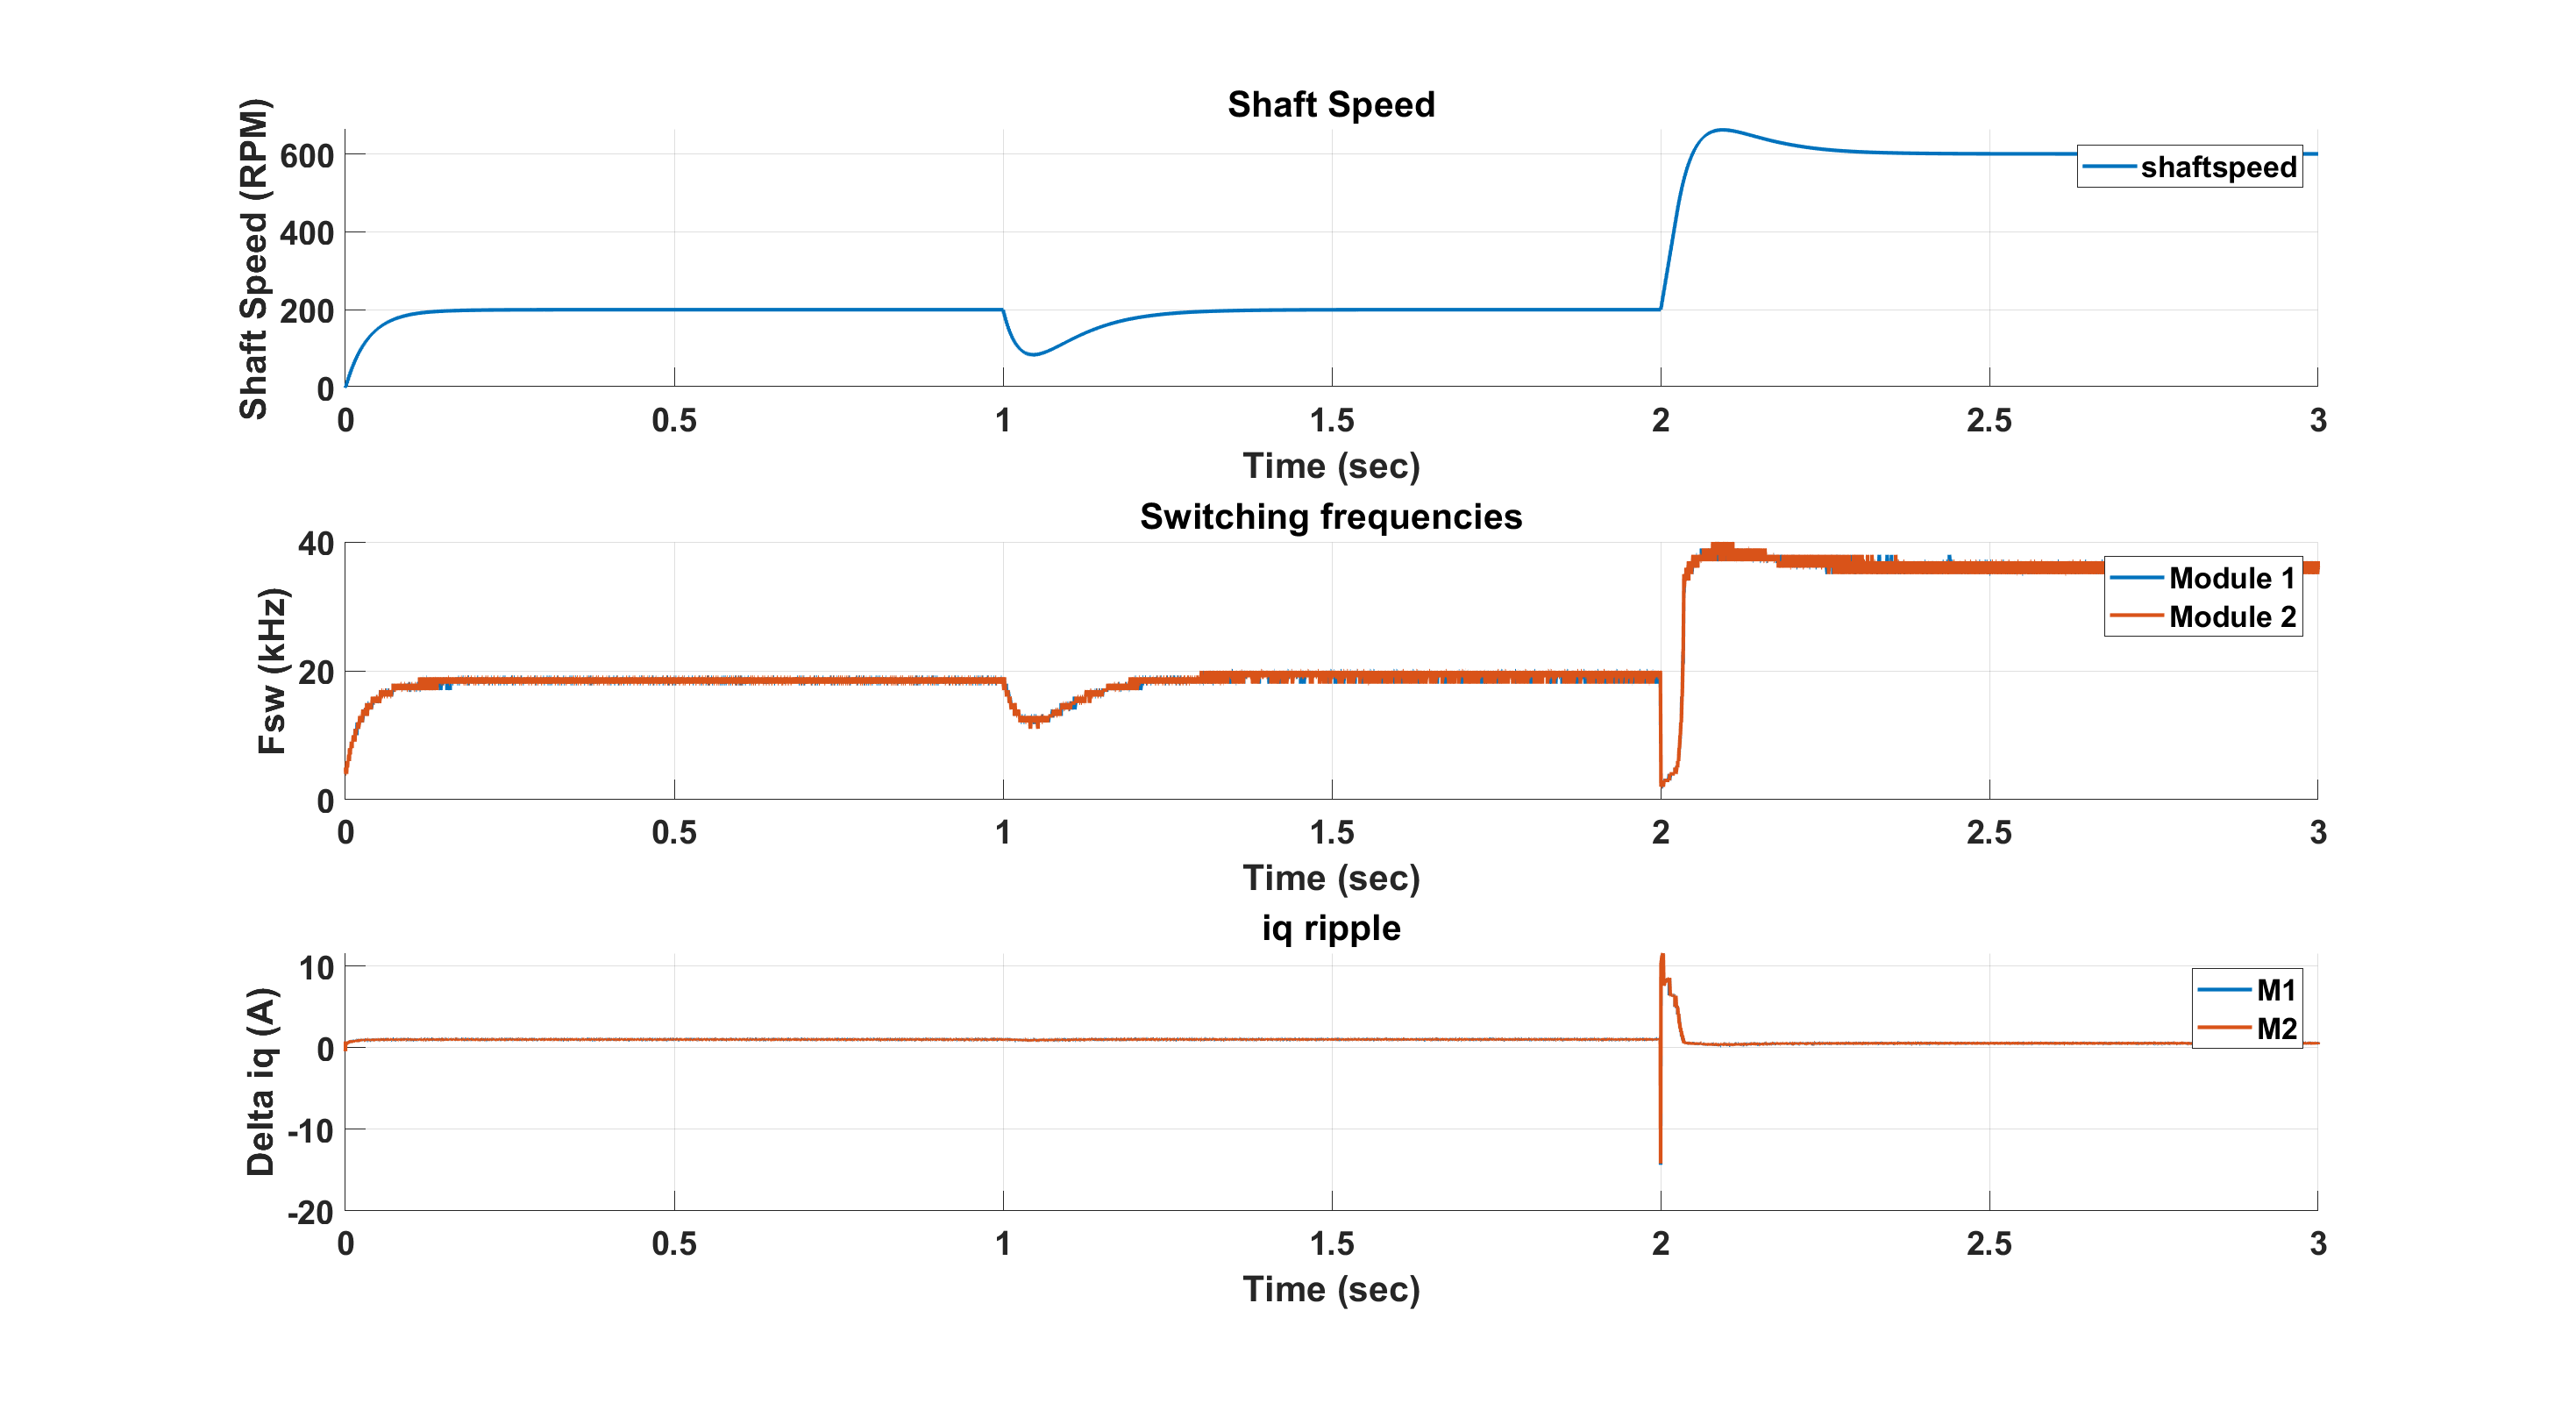
\includegraphics[scale=0.35]{SimulationResults/two_modules/healthy/speed_fsw_iqripple.eps}
\caption{Shaft Speed and Switching Frequency for Healthy Two Modules Operation}
\label{fig:ShaftSpeedFswIqRippleTwoModulesHealthy}
\end{figure}

\begin{figure}[h!]
\centering
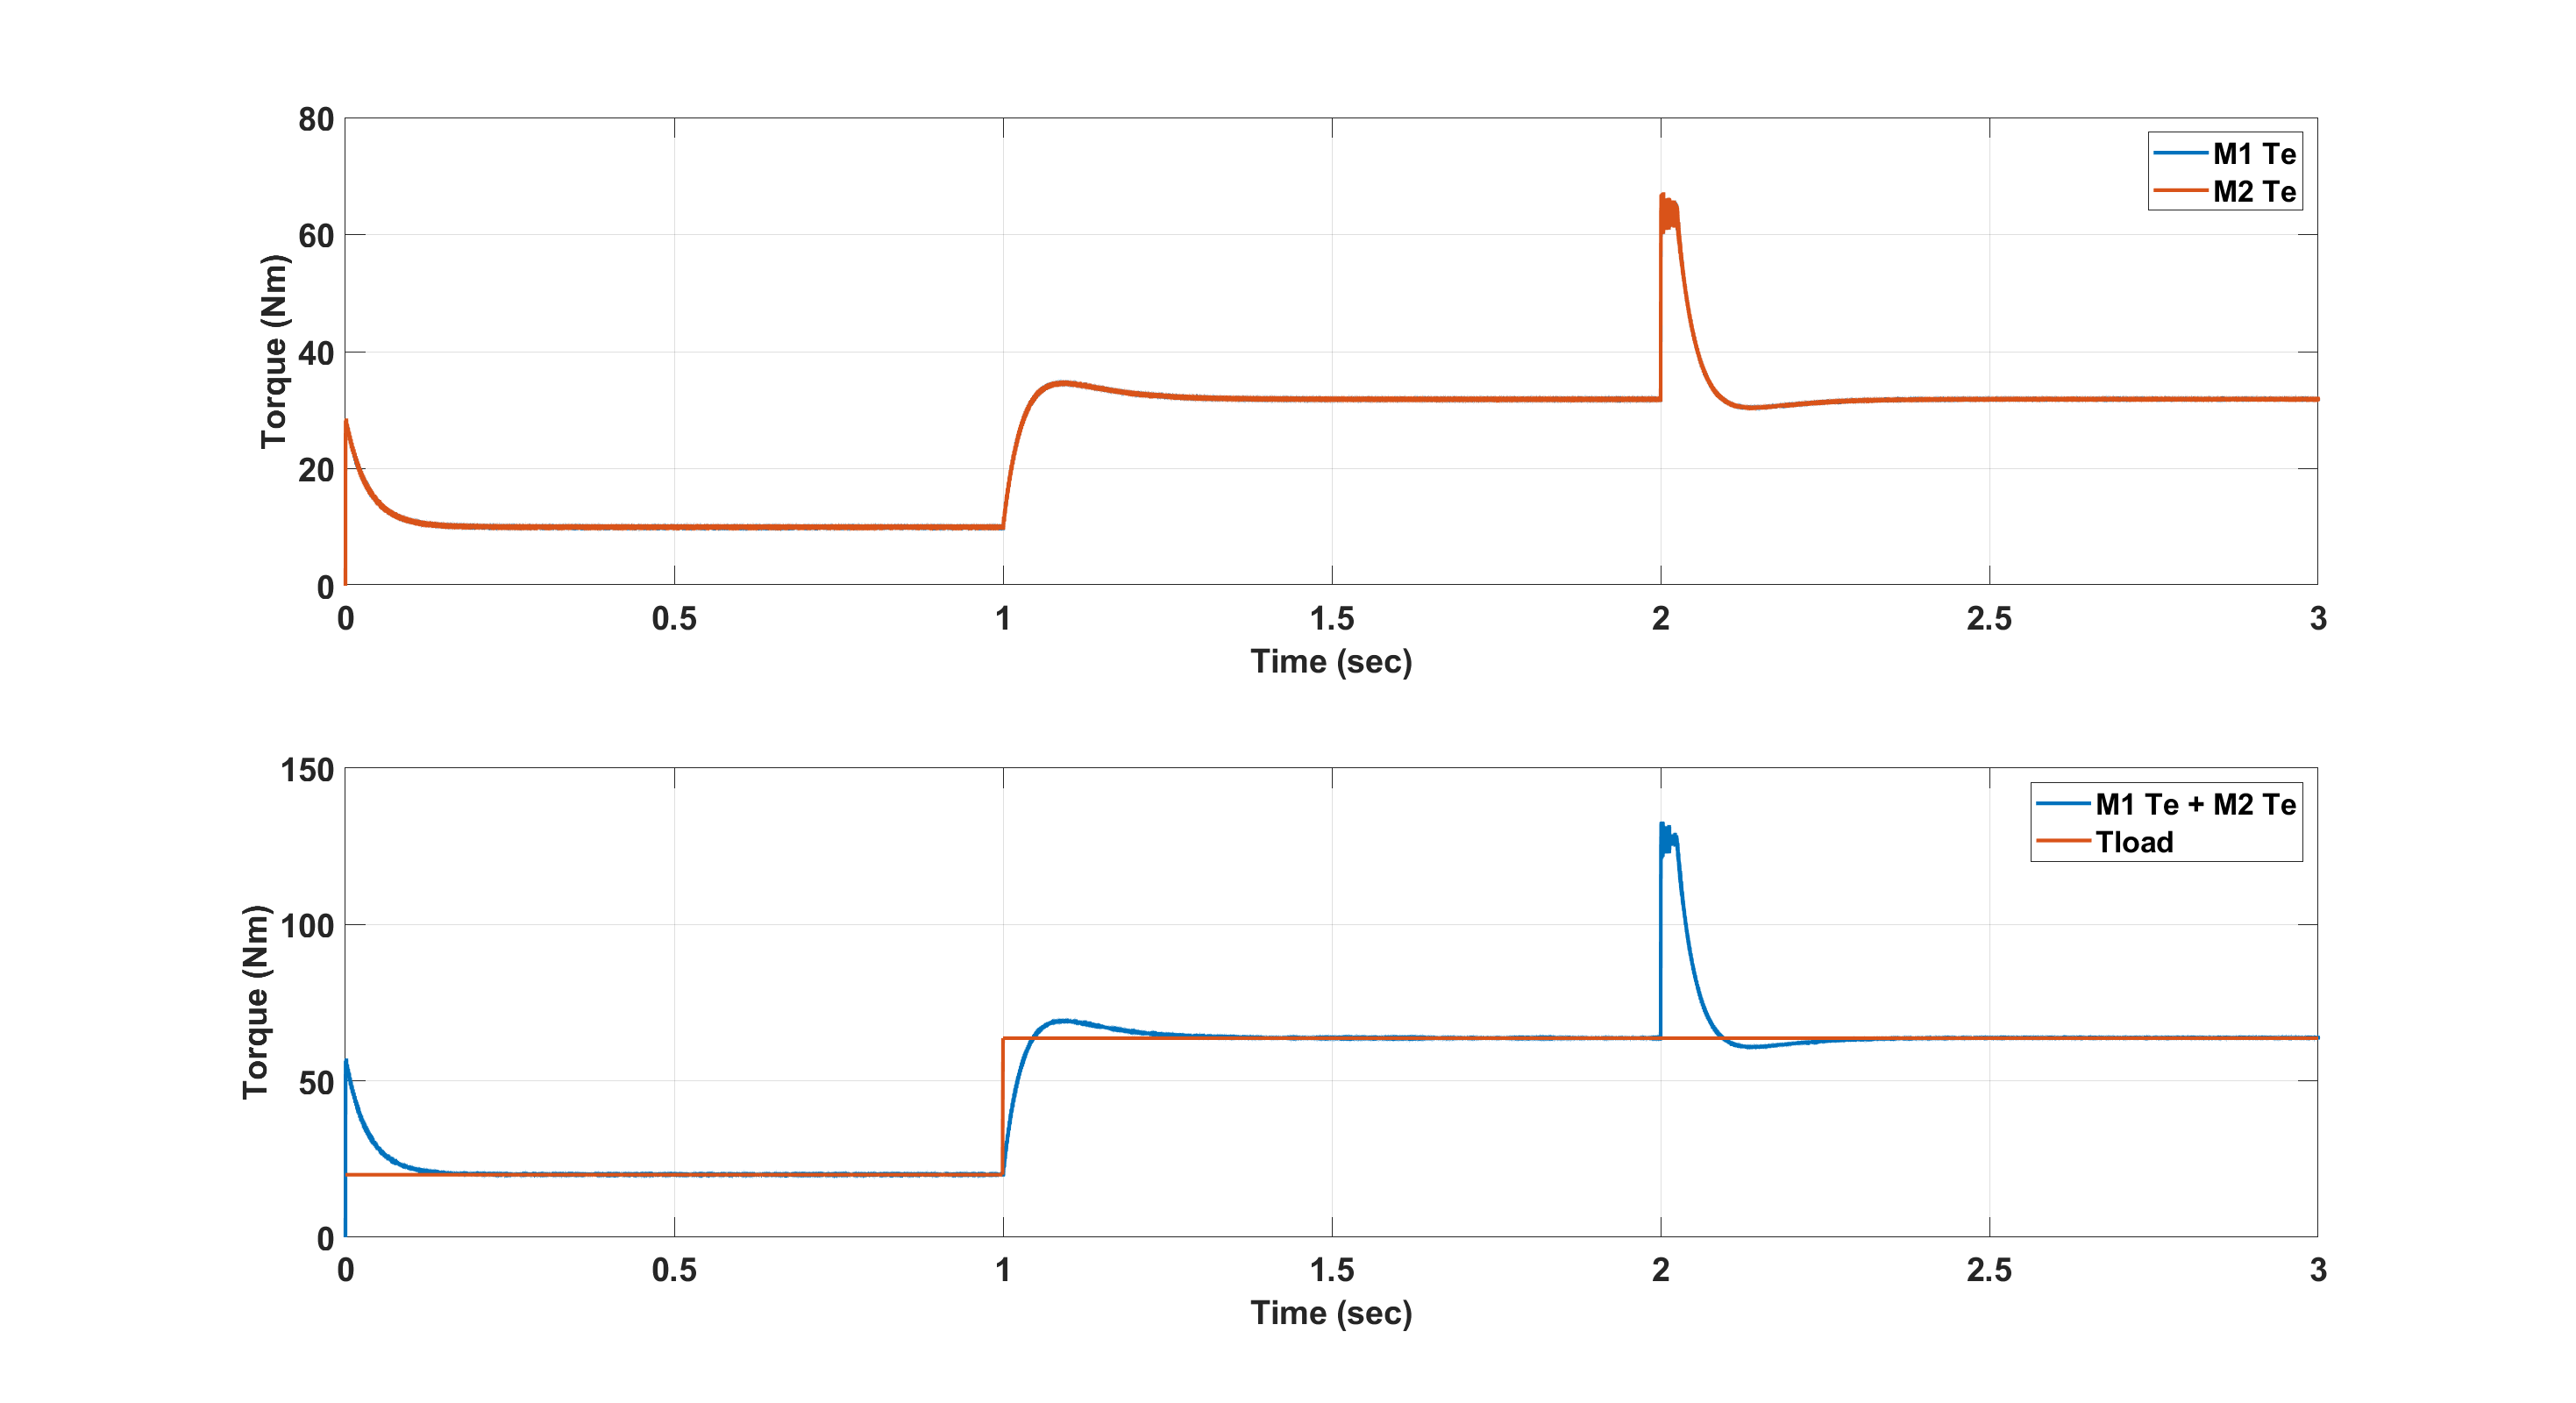
\includegraphics[scale=0.35]{SimulationResults/two_modules/healthy/tref_tload.eps}
\caption{Torque Waveform for Healthy Two Modules Operation}
\label{fig:TorqueTwoModulesHealthy}
\end{figure}


\subsection{Faulty Operation}


\bibliographystyle{plain}
\bibliography{references}
\end{document}
